\documentclass[11pt,a4paper,oneside]{report}

% thanks to http://tex.stackexchange.com/a/47579/71109
\usepackage{ifxetex}
\usepackage{ifluatex}
\newif\ifxetexorluatex % a new conditional starts as false
\ifnum 0\ifxetex 1\fi\ifluatex 1\fi>0
  \xetexorluatextrue
\fi

\ifxetexorluatex
  \usepackage{fontspec}
\else
  \usepackage[T1]{fontenc}
  \usepackage[utf8]{inputenc}
  \usepackage[lighttt]{lmodern}
\fi

\usepackage[english,magyar]{babel} % Alapértelmezés szerint utoljára definiált nyelv lesz aktív, de később külön beállítjuk az aktív nyelvet.

%\usepackage{cmap}
\usepackage{amsfonts,amsmath,amssymb} % Mathematical symbols.
%\usepackage[ruled,boxed,resetcount,linesnumbered]{algorithm2e} % For pseudocodes. % beware: this is not compatible with LuaLaTeX, see http://tex.stackexchange.com/questions/34814/lualatex-and-algorithm2e
\usepackage{booktabs} % For publication quality tables for LaTeX
\usepackage{graphicx}

%\usepackage{fancyhdr}
%\usepackage{lastpage}

\usepackage{anysize}
%\usepackage{sectsty}
\usepackage{setspace} % For setting line spacing

\usepackage[unicode]{hyperref} % For hyperlinks in the generated document.
\usepackage[pdftex,dvipsnames,table]{xcolor}  % Coloured text etc.
\usepackage{listings} % For source code snippets.

\usepackage[amsmath,thmmarks]{ntheorem} % Theorem-like environments.

\usepackage[hang]{caption}

\singlespacing

\newcommand{\selecthungarian}{
  \selectlanguage{magyar}
  \setlength{\parindent}{2em}
  \setlength{\parskip}{0em}
  \frenchspacing
}

\newcommand{\selectenglish}{
  \selectlanguage{english}
  \setlength{\parindent}{0em}
  \setlength{\parskip}{0.5em}
  \nonfrenchspacing
  \renewcommand{\figureautorefname}{Figure}
  \renewcommand{\tableautorefname}{Table}
  \renewcommand{\partautorefname}{Part}
  \renewcommand{\chapterautorefname}{Chapter}
  \renewcommand{\sectionautorefname}{Section}
  \renewcommand{\subsectionautorefname}{Section}
  \renewcommand{\subsubsectionautorefname}{Section}
}

\usepackage[numbers]{natbib}
\usepackage{xspace}

% Personal
\usepackage{tikz}
\usepackage{physics} % Braket notation
\usepackage{dsfont} % Mathds
\usepackage{xargs} % Use more than one optional parameter in a new commands
\usepackage[colorinlistoftodos,prependcaption,textsize=tiny]{todonotes} % Todo notes.
\newcommandx{\unsure}[2][1=]{\todo[inline,size=\normalsize,linecolor=red,backgroundcolor=red!25,bordercolor=red,#1]{#2}}
\newcommandx{\change}[2][1=]{\todo[inline,size=\normalsize,linecolor=blue,backgroundcolor=blue!25,bordercolor=blue,#1]{#2}}
\newcommandx{\info}[2][1=]{\todo[inline,size=\normalsize,linecolor=OliveGreen,backgroundcolor=OliveGreen!25,bordercolor=OliveGreen,#1]{#2}}

%TODO Set the main variables
\newcommand{\vikszerzoVezeteknev}{Nemkin}
\newcommand{\vikszerzoKeresztnev}{Viktória}

\newcommand{\vikkonzulensAMegszolitas}{dr.~}
\newcommand{\vikkonzulensAVezeteknev}{Friedl}
\newcommand{\vikkonzulensAKeresztnev}{Katalin}

\newcommand{\vikcim}{Simulation of quantum walks\\on a classical computer}
\newcommand{\viktanszek}{\bmeszit}
\newcommand{\vikdoktipus}{\msc}

%--------------------------------------------------------------------------------------
% TDK-specifikus változók
%--------------------------------------------------------------------------------------
\newcommand{\tdkev}{2021} % A dolgozat írásának éve (pl. "2014") (Ez OTDK-nál eltérhet az aktuális évtől.)

% További adatok az OTDK címlaphoz (BME-s TDK-hoz nem kell kitölteni)
\newcommand{\tdkevfolyamA}{II} % Első szerző évfolyama, római számmal (pl. IV).
\newcommand{\tdkkonzulensbeosztasA}{egyetemi docens} % Első konzulens beosztása (pl. egyetemi docens)

\newcommand{\szerzoMeta}{\vikszerzoVezeteknev{} \vikszerzoKeresztnev}

%--------------------------------------------------------------------------------------
% Elnevezések
%--------------------------------------------------------------------------------------
\newcommand{\bme}{Budapest University of Technology and Economics}
\newcommand{\vik}{Faculty of Electrical Engineering and Informatics}

\newcommand{\bmeszit}{Department of Computer Science and Information Theory}

\newcommand{\keszitette}{Author}
\newcommand{\konzulens}{Advisor}

\newcommand{\bsc}{Bachelor's Thesis}
\newcommand{\msc}{Master's Thesis}
\newcommand{\tdk}{Scientific Students' Association Report}
\newcommand{\bsconlab}{BSc Project Laboratory}
\newcommand{\msconlabi}{MSc Project Laboratory 1}
\newcommand{\msconlabii}{MSc Project Laboratory 2}

\newcommand{\pelda}{Example}
\newcommand{\definicio}{Definition}
\newcommand{\tetel}{Theorem}

\newcommand{\bevezetes}{Introduction}
\newcommand{\koszonetnyilvanitas}{Acknowledgements}
\newcommand{\fuggelek}{Appendix}

% Optional custom titles
%\addto\captionsenglish{%
%\renewcommand*{\listfigurename}{Your list of figures title}
%\renewcommand*{\listtablename}{Your list of tables title}
%\renewcommand*{\bibname}{Your bibliography title}
%}

\newcommand{\szerzo}{\vikszerzoKeresztnev{} \vikszerzoVezeteknev}
\newcommand{\vikkonzulensA}{\vikkonzulensAMegszolitas\vikkonzulensAKeresztnev{} \vikkonzulensAVezeteknev}
\newcommand{\vikkonzulensB}{\vikkonzulensBMegszolitas\vikkonzulensBKeresztnev{} \vikkonzulensBVezeteknev}
\newcommand{\vikkonzulensC}{\vikkonzulensCMegszolitas\vikkonzulensCKeresztnev{} \vikkonzulensCVezeteknev}

\newcommand{\selectthesislanguage}{\selectenglish}

\bibliographystyle{plainnat}

\newcommand{\ie}{i.e.\@\xspace}
\newcommand{\Ie}{I.e.\@\xspace}
\newcommand{\eg}{e.g.\@\xspace}
\newcommand{\Eg}{E.g.\@\xspace}
\newcommand{\etal}{et al.\@\xspace}
\newcommand{\etc}{etc.\@\xspace}
\newcommand{\vs}{vs.\@\xspace}
\newcommand{\viz}{viz.\@\xspace} % videlicet
\newcommand{\cf}{cf.\@\xspace} % confer
\newcommand{\Cf}{Cf.\@\xspace}
\newcommand{\wrt}{w.r.t.\@\xspace} % with respect to
\newcommand{\approximately}{approx.\@\xspace}

\newcommand{\appendixnumber}{1}  % a fofejezet-szamlalo az angol ABC 1. betuje (A) lesz

% Page layout setup
\pagestyle{plain}
\marginsize{35mm}{25mm}{15mm}{15mm}
\setcounter{tocdepth}{3}
\setcounter{secnumdepth}{3}

% Margón túllógó sorok tiltása.
\sloppy
% A fattyú- és árvasorok elkerülése.
\widowpenalty=10000
\clubpenalty=10000

% Kötőjeles szavak elválasztásának engedélyezése
\def\hyph{-\penalty0\hskip0pt\relax}

% Setup hyperref package
\hypersetup{
    % bookmarks=true,          % show bookmarks bar?
    unicode=true,              % non-Latin characters in Acrobat's bookmarks
    pdftitle={\vikcim},        % title
    pdfauthor={\szerzoMeta},   % author
    pdfsubject={\vikdoktipus}, % subject of the document
    pdfcreator={\szerzoMeta},  % creator of the document
    pdfproducer={},            % producer of the document
    pdfkeywords={},            % list of keywords (separate then by comma)
    pdfnewwindow=true,         % links in new window
    colorlinks=true,           % false: boxed links; true: colored links
    linkcolor=black,           % color of internal links
    citecolor=black,           % color of links to bibliography
    filecolor=black,           % color of file links
    urlcolor=black             % color of external links
}

% Set up listings
\definecolor{lightgray}{rgb}{0.95,0.95,0.95}
\lstset{
	basicstyle=\scriptsize\ttfamily, % print whole listing small
	keywordstyle=\color{black}\bfseries, % bold black keywords
	identifierstyle=, % nothing happens
	% default behavior: comments in italic, to change use
	% commentstyle=\color{green}, % for e.g. green comments
	stringstyle=\scriptsize,
	showstringspaces=false, % no special string spaces
	aboveskip=3pt,
	belowskip=3pt,
	backgroundcolor=\color{lightgray},
	columns=flexible,
	keepspaces=true,
	escapeinside={(*@}{@*)},
	captionpos=b,
	breaklines=true,
	frame=single,
	float=!ht,
	tabsize=2,
	literate=*
		{á}{{\'a}}1	{é}{{\'e}}1	{í}{{\'i}}1	{ó}{{\'o}}1	{ö}{{\"o}}1	{ő}{{\H{o}}}1	{ú}{{\'u}}1	{ü}{{\"u}}1	{ű}{{\H{u}}}1
		{Á}{{\'A}}1	{É}{{\'E}}1	{Í}{{\'I}}1	{Ó}{{\'O}}1	{Ö}{{\"O}}1	{Ő}{{\H{O}}}1	{Ú}{{\'U}}1	{Ü}{{\"U}}1	{Ű}{{\H{U}}}1
}

% Set up theorem-like environments

\theoremseparator{.}
\theorembodyfont{\upshape}
\newtheorem{example}{\pelda}
\newtheorem{property}{\tulajdonsag}
\newtheorem{definition}{\definicio}
\newtheorem{theorem}{\tetel}
\numberwithin{example}{chapter}
\numberwithin{property}{chapter}
\numberwithin{definition}{chapter}
\numberwithin{theorem}{chapter}

\newcommand{\lineparagraph}[1]{\paragraph{#1}\mbox{}\\}
\newcommand{\linesubparagraph}[1]{\subparagraph{#1}\mbox{}\\}

% Setup captions
\captionsetup[figure]{
	width=.75\textwidth,
	aboveskip=10pt}

\renewcommand{\captionlabelfont}{\bf}
\renewcommand{\captionfont}{\footnotesize\it}

% Hyphenation exceptions
\hyphenation{Shakes-peare Mar-seilles ár-víz-tű-rő tü-kör-fú-ró-gép}

\author{\vikszerzo}
\title{\viktitle}

\begin{document}

\pagenumbering{gobble}
\selectthesislanguage
%% TDK címlap
\begin{titlepage}
  \begin{center}  
  
\includegraphics[width=7cm]{./figures/bme_logo.pdf}
  \vspace{0.3cm}
  
  \bme \\
  \vik \\
  \viktanszek \\
  \vspace{5cm}
  
  \huge {\vikcim}
  \vspace{1.5cm}
  
  \large {\textbf{\tdk}}
  \vfill
    
  {\Large 
  	\keszitette: \\ \vspace{0.3cm}
  	\szerzo \\
  	\vspace{1.5cm}
  	\konzulens: \\ \vspace{0.3cm}
  	\vikkonzulensA \\
  }
  
  \vspace{2cm}
  \large {\tdkev}
 \end{center}
\end{titlepage}
%% Címlap vége

\tableofcontents\vfill
\listoftodos[Notes]\vfill

\pagenumbering{roman}
\setcounter{page}{1}

\selecthungarian

%----------------------------------------------------------------------------
% Abstract in Hungarian
%----------------------------------------------------------------------------
\chapter*{Kivonat}\addcontentsline{toc}{chapter}{Kivonat}

TODO: Magyarra fordítás


\vfill
\selectenglish


%----------------------------------------------------------------------------
% Abstract in English
%----------------------------------------------------------------------------
\chapter*{Abstract}\addcontentsline{toc}{chapter}{Abstract}

Bioinformatics is an interdisciplinary field between computer science and biology. Its main goal is to answer biological questions by transforming them into computational problems and providing efficient algorithmic solutions to them. Researching bioinformatics has a significant impact on our everyday lives since discoveries in this area can help us solve many of today's major global problems, for example, aiding the creation of more effective medical treatments, advancing our understanding of genetic diseases, developing resistant crops to tackle a global food crisis or inventing novel technologies to reduce and revert environmental pollution.

Unfortunately, many of the applicable problems in bioinformatics turn out to be computationally hard problems. Despite all the research effort, no sufficiently fast, deterministic solutions were found to these problems with the current limitations of our hardware.

In recent years, the field of quantum informatics has experienced increased attention from governmental entities and global corporations, who invested significantly into designing new types of hardware based on quantum physical phenomena and developing complementary software capable of solving previously challenging problems. While quantum computing research is still in its early stages and the limits of quantum hardware are unknown, the availability of this different computational model has allowed new forms of algorithmic design to emerge, with promising theoretical results.

\vfill
\selectthesislanguage

\newcounter{romanPage}
\setcounter{romanPage}{\value{page}}
\stepcounter{romanPage}
\pagenumbering{arabic}
\chapter{Introduction}

In recent years, there has been an increasing focus on quantum informatics. Influential global companies such as IBM, Google, Microsoft, and Amazon have invested significant amounts into studying and developing hardware and software for this sector, while the European Union and Hungary have launched several programs to accelerate quantum research.

Current technology is yet to produce a significant number of qubits (quantum bits) in a quantum processor, but many believe the amount will increase over the years. The first practical quantum algorithms to be run on these processors are likely to be the ones that use qubits sparingly. Quantum walking, the generalized version of classical random walking, is exactly this kind of algorithm. The number of qubits required to run a quantum walk on a graph is logarithmic in the number of vertices, making it a promising technique for the near future. Furthermore, Grover's search algorithm (a basis for many quantum algorithms) can be viewed as a special case of quantum walks, which illustrates the potential power of this method.

In my dissertation, I present the mathematical framework for quantum walks, detailing the points critical for implementation, which are given less emphasis in the literature. I describe the architecture and capabilities of the simulator program I have written and the conclusions of the simulations I have run.

I developed the software using Python 3, based on the Strategy design pattern. It supports graphs commonly found in the literature while also providing a method for combining them, facilitating experimentation on several kinds of regular graphs. This composition is also the foundation of the quantum walk. It can simulate classical and quantum walks on the same graphs and produce a report file detailing the results. In the quantum case, the characteristics of the walk are also dependent on the type of coin used to generate the probabilities, which can be defined in several ways. The program includes the Hadamard, Grover, and Fourier coins and can easily be extended with others.

Running several simulations, I compared the behavior of classical and quantum walks and demonstrated the quantum characteristics expected from the theoretical literature, the ballistic nature of the Hadamard walk, and the cyclic property of quantum walks.

Classical random walks are well-known tools for describing different stochastic processes. Many real-life scientific approaches rely on these methods, including stock price movement prediction, natural language processing, Brownian motion description; and evolution, population and disease outbreak models. Other algorithms utilize random walks to gain speed or combat the search space's scale, most notably Google's Page Rank algorithm and various recommender systems.~\cite{XiaReview}.

In recent years quantum computing has been gaining traction amongst researchers and computer scientists. While there exists a wide variety of quantum algorithms to be explored, I specifically targeted quantum walks due to their reasonable hardware requirements and promising features. Quantum walks provide a quadratic speedup compared to their classical counterparts and display behaviour, such as the ballistic nature and the cyclic property that their classical equivalent does not, while only requiring logarithmic space, which due to the various limitations of physical qubit realization is particularly valuable.~\cite{Portugal}

Since currently, the publicly available quantum computers can operate with only around 5-10 qubits, I created a simulator software that runs on a regular computer to experiment with the algorithm. I am hopeful that the time for feasibly switching to quantum hardware is just around the corner.

During my research, I have observed a significant lack of software engineering perspective on this subject. Most research papers are written by physicists who are well acquainted with the details of quantum mechanics with a heavy focus on physics-related formulas and functional descriptions. It has been a strenuous process to gather the motivation and justification of certain implementation choices that seem to be the standard for someone in the inner circle but strange for me, just getting started with the topic.

This report aims to provide a comprehensible introduction to quantum walking from the software engineer's perspective, spending extra effort on implementation-specific details and mathematical proofs missing from the available literature. In contrast with the functional descriptions, I describe the algorithms using linear algebra, allowing for a more natural way to implement the simulation.

The rest of this report is structured in the following way: In Chapters 2 and 3, I briefly introduce classical random walks and quantum computing, using only the necessary formulas and focusing on the details employed later in the report. In Chapter 4, I introduce quantum walking in a bottom-up approach, starting from the simplest form and then generalizing it. Contrary to many authors, I use linear algebra exclusively to describe each step since implementation on a universal quantum computer requires the definition to come in the form of unitary transformations.

Section 4.3 discusses two of the generalization techniques found in~\cite{Portugal}. I present my improvement to one of these methods, which I have proven to have the equivalent result but remove an exponential memory requirement from the implementation. The other method in~\cite{Portugal} uses a constraint about the evolution operator, for which I have not found proof in the literature. Here, I present my more generalized version of this constraint and the proof I have given.

In Chapter 5, I describe the architecture and implementation details of my simulator software, then in Chapter 6, I present the results obtained from my simulation runs.
\section{Classical random walks}

A classical random walk describe a stohastic process.

\unsure{The sequence can also be regarded as a special category of Markov chain ->Homogenous?}

Classical random walks on graphs can be defined using Markov-chains. Markov-chains
are well explained in Leo Breiman's book on Probability\cite{breiman_probability_1992} and Feng Xia, Senior Member, IEEE, Jiaying Liu, Hansong Nie, Yonghao Fu, Liangtian Wan, Member, IEEE,
Xiangjie Kong, Senior Member, IEEE - Random Walks: A Review of Algorithms and Applications, from IEEE Transactions on emerging topics in computational intelligence, on May 2019.

(Információelmélet előadás / a könyvet be lehetne idézni, bár kevésbé szeretik)

\definition{\textbf{Markov-chain}} (First order, discrete-time, discrete-space) A Markov-chain is a sequence of independent random variables from the same distribution, $X_1, X_2, X_3, \dots$, (with value set $A$), that have the Markov property:

\unsure{Hogy kellene az értékkészletet ($A$) jelölni?}

$P(X_k = x_k | X_{k-1} = x_{k-1}, \dots, X_1 = x_1) = P(X_k = x_k | X_{k-1} = x_{k-1})$

$\forall k\geq{}2$ and $x_{1},\dots, x{k}$ from the value set.

\definition{\textbf{Homogenous Markov-chain}} Time invariant, i.e.:
$P(\Phi_k = i | \Phi_{k-1} = j) = p_{j,i}$ $\forall k\geq{}2$, $\forall i,j \in{} A$, which is called the transition probability from $i$ to $j$ and form the transition probability matrix $P$.

This allows us to represent Homogenous Markov-chains as directed graphs.

\definition{\textbf{Distribution of the Markov-chain}} at the $i$th step, the Markov-chain's distribution is the distribution of $X_i$, which is $P(X_i = j)$.

\definition{\textbf{Stacionary distribution}} of the Markov chain is $p_{j} = \lim\limits_{i \to \infty} P(X_i = j)$.

\definition{\textbf{Graph representation of homogenous Markov-chains}}
Graph $G(V,E)$ represents a homogenous Markov-chain $X_1, X_2, X_3, \dots$, (with value set $A$ and transition probability matrix $P$), if $V=A$ and $E(i,j) = p_{j,i}$ $\forall{}i,j\in{}A$.

\definition{\textbf{Random walk on a graph}}
A random walk on this graph $G$ visits the nodes represented by the Markov-chain: $X_1, X_2, X_3, \dots$.


\chapter{Quantum walks}

In classical random walks, the walker moves from the current vertex via one of its outgoing edges, chosen randomly, weighted by the edge weights. This random choice can be interpreted as a (generalized) coin toss.

To formulate a quantum version of graph walking, we define the quantum coin, which will replace the classical concept of randomness with quantum superposition.

\section{Formulating the Quantum coin}

I used Renato Portugal's Quantum Walks and Search Algorithms~\cite{Portugal} book as a reference for the different types of coins I present in this section.

A \textit{quantum coin} is a quantum system, which behaves according to the postulates of quantum mechanics. It has a current state, represented by a state vector in a Hilbert space and a unitary time evolution operator, describing a coin toss.

After tossing the coin, the resulting coin state chooses the next step of the quantum walker. If there are $d$ outgoing edges to choose from, then the coin's state space must have $d$ orthonormal basis states, each corresponding to one of the possible edges. If the current state is one of the basis states, then the walker moves in that direction. However, in the quantum world, the coin can also be in a superposition, consisting of multiple basis states. This means that the walker will simultaneously move in all corresponding directions and occupy more than one vertex at the same time, resulting in the walker spreading over the graph in a superposition.

For the $d$ dimensional coin state, the corresponding coin flip operator is a $(d\times{}d)$ dimensional unitary matrix. Based on what the transition operator is, multiple types of coins can be defined. The following ones are typically used in quantum walks.

\subsection{Hadamard coin}

The Hadamard coin is the most commonly used quantum coin. It is defined by the Hadamard-matrix as a transition operator:

\begin{align*}
  \mathbf{H} = \frac{1}{\sqrt{2}}\begin{pmatrix}
      1 & 1  \\
      1 & -1
    \end{pmatrix}.
\end{align*}

If the starting coin state is $\ket{0}$, then flipping the coin once results in the following state:

\begin{align*}
 \mathbf{H}\ket{0} = \frac{1}{\sqrt{2}}\begin{pmatrix}
      1 & 1  \\
      1 & -1
    \end{pmatrix} \begin{pmatrix} 1 \\ 0 \end{pmatrix}
    = \frac{1}{\sqrt{2}} \begin{pmatrix} 1 \\ 1 \end{pmatrix} = \frac{1}{\sqrt{2}} \ket{0} + \frac{1}{\sqrt{2}} \ket{1}.
\end{align*}

If we measured the above coin, the probability of measuring $0$ is

\begin{align*}
P(0 \mid \frac{1}{\sqrt{2}} (\ket{0} + \ket{1})) =
\left\lvert\frac{1}{\sqrt{2}}\right\rvert^2 =
\frac{1}{2}.
\end{align*}

Similarly, if the starting coin state is $\ket{1}$, then flipping the coin once results in the following state:

\begin{align*}
   \mathbf{H}\ket{1} = \frac{1}{\sqrt{2}}\begin{pmatrix}
      1 & 1  \\
      1 & -1
    \end{pmatrix} \begin{pmatrix} 0 \\ 1 \end{pmatrix}
    = \frac{1}{\sqrt{2}} \begin{pmatrix} 1 \\ -1 \end{pmatrix} = \frac{1}{\sqrt{2}} \ket{0} - \frac{1}{\sqrt{2}} \ket{1}.
\end{align*}

The probability of measuring $1$ here is similarly

\begin{align*}
P(1 \mid \frac{1}{\sqrt{2}} (\ket{0} - \ket{1})) =
\left\lvert-\frac{1}{\sqrt{2}}\right\rvert^2 =
\frac{1}{2}.
\end{align*}

An unexpected feature of this coin comes from the fact, that the Hadamard-matrix is Hermitian (self-adjoint), i.e. $\mathbf{H}^{\dagger} = \mathbf{H}$, while also unitary, i.e. $\mathbf{H}^{\dagger} = \mathbf{H}^{-1}$, which results in $\mathbf{H}^{-1} = \mathbf{H}$, thus $\mathbf{H}\mathbf{H} = \mathbf{I}$. This means, that after flipping the coin twice without measuring it, it will return the coin state to its origin. For example, starting from $\ket{0}$:

\begin{align*}
 \mathbf{H}^2 \ket{0} = \mathbf{H}\frac{1}{\sqrt{2}}(\ket{0} + \ket{1}) = \frac{1}{2}(\ket{0} + \ket{1} + \ket{0} - \ket{1}) = \ket{0}.
\end{align*}

After the second flip, the probability of measuring $\ket{0}$ is $1$, due to the destructive interference between the two $\ket{1}$ probability amplitudes, demonstrating a significant contrast between classical and quantum walks.

\begin{definition}[$2^n$ dimensional Hadamard-coin]

A $2^n$ dimensional Hadamard-coin operator can be created by taking the tensor product of the $2$ dimensional Hadamard-coin $n$ times: $\mathbf{H}^{\otimes{}n}$.

\end{definition}

\subsection{Grover coin}

The Grover coin originates from Grover's search algorithm, where it is applied as the diffusion operator.

Let $\ket{D}$ be the following state:

\begin{align*}
\ket{D} = \mathbf{H}^{\otimes{}n}\ket{0} =
\frac{1}{\sqrt{2^n}} \sum\limits_{i=0}^{2^n-1} \ket{i}.
\end{align*}

Using $\ket{D}$, the Grover coin is the following unitary matrix:

\begin{align*}
    \mathbf{G} = 2\ket{D}\bra{D} - \mathbf{I}.
\end{align*}

If $N = 2^n$, then $\mathbf{G}$ unrolls to the following representation:

\begin{align*}
  \mathbf{G} = \begin{pmatrix}
      \frac{2}{N} - 1 & \frac{2}{N} & \dots  & \frac{2}{N} \\
      \frac{2}{N} & \frac{2}{N} - 1 & \dots  & \frac{2}{N} \\
      \vdots & \vdots & \ddots & \vdots \\
      \frac{2}{N} & \frac{2}{N} & \ddots & \frac{2}{N} - 1
    \end{pmatrix}.
\end{align*}

\subsection{Fourier coin}

In contrast to the Hadamard and Grover coins, the Fourier coin can be of any size, not just a power of 2. A size $N$ Fourier-coin, $F_N$ is defined by the matrix of the Quantum Fourier Transform:

\begin{align*}
\mathbf{F}[k,l] = \frac{1}{\sqrt{N}} \omega^{kl}
\end{align*}

where $\omega$ is the $N$-th root of unity,

\begin{align*}
\omega = e^{\frac{2\pi{}i}{N}}.
\end{align*}

$\mathbf{F}$ unrolls to the following representation:

\begin{align*}
\mathbf{F} = \frac{1}{\sqrt{N}}
\begin{pmatrix}
  1 & 1 & 1 & \dots & 1 \\
  1 & \omega & \omega^2 & \dots & \omega^{N-1} \\
  1 & \omega^2 & \omega^4 & \dots & \omega^{2(N-1)} \\
  \vdots & \vdots & \vdots & \ddots & \vdots \\
  1 & \omega^{N-1} & \omega^{2(N-1)} & \dots & \omega^{(N-1)(N-1)}
\end{pmatrix}
\end{align*}

\section{Quantum walks on the line}

Kempe introduces quantum walks from a physicist's perspective in~\cite{KempeIntroduction} using a particle characterised by its position on the line $\ket{x}$ and its spin state $\ket{s}$.

\subsection{State space}

\lineparagraph{Spin state}

The spin state is in $H_2$ with the basis states spin up and down:

\begin{align*}
\ket{\uparrow} = \ket{0}, \\
\ket{\downarrow} = \ket{1}.
\end{align*}

The spin state vector is then given by:

\begin{align*}
\ket{s} = s_0 \ket{\uparrow} + s_1 \ket{\downarrow}.
\end{align*}

\lineparagraph{Position state}

At the start of the walk the particle is at the origin $\ket{0}$ and the walking lasts for $N$ steps. The position state is in $H_{(2N+1)}$ with the following basis vectors corresponding to the possible positions on the line.

\begin{align*}
\{
\ket{-N},\ket{-(N-1)},\dots,
\ket{-1},\ket{0},\ket{1},\dots,
\ket{N-1},\ket{N}
\}
\end{align*}

I index the basis states using negative numbers to match the labels on the axis.

The position state vector is then given by:

\begin{align*}
    \ket{x} = \sum\limits_{i=-N}^{N}x_i\ket{i}.
\end{align*}

\lineparagraph{Composite state}

The composite state of the system, according to \hyperref[PostulateIV]{[PostulateIV]} is then

\begin{align*}
    \ket{x}\otimes{}\ket{s}.
\end{align*}

\subsection{Evolution}

The particle travels on the line based on its current spin state:
\begin{itemize}
\item If the current spin state is $\ket{0}$, the particle moves to the left, i.e. from position $\ket{i}$ the particle travels to position $\ket{i-1}$.
\item If the current spin state is $\ket{1}$, the particle moves to the right, i.e. from position $\ket{i}$ the particle travels to position $\ket{i+1}$.
\end{itemize}

This step is realised with the unitary matrix $\mathbf{S}$ which operates on the complete state of the system, $\ket{x}\otimes{}\ket{s}$ and is assembled from a left and a right shift operator acting on $\ket{x}$ and another operator for checking $\ket{s}$ compiled using tensor product.

\begin{definition}[Left shift operator]

To move from position $\ket{i}$ to the left ($\ket{i-1}$) the position vector is multiplied with the following $\mathbf{L}$ matrix, containing $1$'s above the diagonal. To keep $\mathbf{S}$ unitary, an unused transition must be added in the lower left corner.

\change{Előrehivatkozni a permutációmátrixos tételre.}

\begin{align}
\label{LeftShift}
\mathbf{L} = \ket{N}\bra{-N} + \sum\limits_{i=-(N-1)}^{N} \ket{i-1}\bra{i} =
\left(
    \begin{array}{ccccc}
        0      & 1      & 0      & \cdots & 0      \\
               & \ddots & \ddots & \ddots & \vdots \\
        \vdots &        & \ddots & \ddots & 0      \\
        0      &        &        & \ddots & 1      \\
        1      & 0      & \cdots &        & 0
      \end{array}
\right)
\end{align}

For a given basis vector $\ket{j}$ only one of the summands in $\mathbf{L}$ is non-zero, where $i=j$, resulting in the required shift being performed.

\begin{align*}
\mathbf{L}\ket{j} = \ket{j-1}\bra{j}\ket{j} = \ket{j-1}
\end{align*}

\end{definition}

\begin{definition}[Right shift operator]

To move from position $\ket{i}$ to the right ($\ket{i+1}$) the position vector is multiplied with the following $\mathbf{R}$ matrix, containing $1$'s under the diagonal. To keep $\mathbf{S}$ unitary, an unused transition must be added in the top right corner.

\change{Előrehivatkozni a permutációmátrixos tételre.}

\begin{align}
\label{RightShift}
\mathbf{R} = \ket{-N}\bra{N} + \sum\limits_{i=-N}^{N-1} \ket{i+1}\bra{i} =
\left(
    \begin{array}{ccccc}
        0      &        & \cdots & 0      & 1      \\
        1      & \ddots &        &        & 0      \\
        0      & \ddots & \ddots &        & \vdots \\
        \vdots & \ddots & \ddots & \ddots &        \\
        0      & \cdots & 0      & 1      & 0
      \end{array}
\right)
\end{align}

For a given basis vector $\ket{j}$ only one of the summands in $\mathbf{R}$ is non-zero, where $i=j$, resulting in the required shift being performed.

\begin{align*}
\mathbf{R}\ket{j} = \ket{j+1}\bra{j}\ket{j} = \ket{j+1}
\end{align*}

\end{definition}

\lineparagraph{Shift operator}

Using matrixes $L$ and $R$ operating on the position register $\ket{x}$ only, we construct a unitary operator $S$, which operates on the composite state of the system, $\ket{x} \otimes \ket{s}$, executing matrix $\mathbf{L}$ on $\ket{x}$ only when $\ket{s} = \ket{0}$ and matrix $\mathbf{R}$ only when $\ket{s}=\ket{1}$.

\begin{align}
\label{ShiftOperator}
  \mathbf{S} = \mathbf{L}\otimes\ket{0}\bra{0} + \mathbf{R}\otimes\ket{1}\bra{1}
\end{align}

The execution logic is as follows:

\begin{gather*}
    \mathbf{S}(\ket{x}\otimes{}\ket{s}) = \\
    (\mathbf{L}\otimes\ket{0}\bra{0} + \mathbf{R}\otimes\ket{1}\bra{1})(\ket{x}\otimes{}\ket{s}) = \\ (\mathbf{L}\otimes\ket{0}\bra{0})(\ket{x}\otimes{}\ket{s}) + (\mathbf{R}\otimes\ket{1}\bra{1})(\ket{x}\otimes{}\ket{s}) = \dots
\end{gather*}

using \hyperref[TensorMixedProduct]{[TensorMixedProduct]}:

\begin{gather*}
    \dots = \mathbf{L}\ket{x}\otimes(\ket{0}\bra{0}\ket{s}) + \mathbf{R}\ket{x}\otimes(\ket{1}\bra{1}\ket{s}) = \\
    \ket{x-1}\otimes{}s_0\ket{0} + \ket{x+1}\otimes{}s_1\ket{1} = \\
    s_0\ket{x-1, 0} + s_1\ket{x+1,1}.
\end{gather*}

\begin{itemize}
\item If the spin state was $\ket{s} = \ket{0}$ at the beginning, then $s_0=1$ and $s_1=0$, which means that the resulting system state is $\ket{x-1,0}$, which means that the particle shifted to the left, as designed.
\item If the spin state was $\ket{s} = \ket{1}$ at the beginning, then $s_0=0$ and $s_1=1$, which means that the resulting system state is $\ket{x+1,1}$, which means that the particle shifted to the right, also as intended.
\end{itemize}

Furthermore, the spin state can be any mixed state $s_0\ket{0} + s_1\ket{1}$ as well. In this case the particle will shift \textit{both} to the left and to the right, at the same time. When measured, the particle can be found in position $\ket{x-1}$ with probability $|s_0|^2$ and in position $\ket{x+1}$ with probability $|s_1|^2$.

In quantum graph walks, the walker can simultaneously explore multiple parallel paths in the graph, at the same time. With good design, this behaviour can be used to search the graph faster than in classical random graph walks.

\lineparagraph{Coin operator}

To inject the quantum superposition into the walk, the particle's spin state is transformed using any $2$ dimensional unitary matrix between shift operations. The Hadamard, Grover and Fourier coins mentioned earlier are commonly used as coin operators.

For any $C$ operator on the coin register, the unitary transform for the composite system is defined as follows:

\begin{align*}
    \mathbf{\hat{C}} = \mathbf{I} \otimes \mathbf{C}
\end{align*}

since the coin operator does not modify the position register.

\lineparagraph{Evolution operator}

Combining the shift operator and the coin operator together, we obtain the following evolution operator, defining one step of the quantum walk on the line. The step consists of flipping the coin once, then applying the shifting the walker's position accordingly, as follows:

\begin{align*}
    \mathbf{U} = \mathbf{S}\mathbf{\hat{C}} = \mathbf{S}(\mathbf{I}\otimes{}\mathbf{C})
\end{align*}

\subsection{Measurement}

To measure the probability of the particle being at position $\ket{i}$, the projective measurement operator acting on $\ket{x}$ is defined as $\mathbf{P_i} = \ket{i}\bra{i}$, in accordance with \hyperref[PostulateIIIProjective]{[PostulateIIIProjective]}.

Since the coin register need not be measured, we apply the identity operator on it, using $\mathbf{P_i} \otimes \mathbf{I}$ on the complete system to measure the particle's current position.

The probability of finding the particle in position $i$ is:

\begin{gather*}
    P(i | \ket{x}) = \bra{x,s}\mathbf{P_i}\otimes{}\mathbf{I}\ket{x,s} = \dots
\end{gather*}

using \hyperref[TensorMixedProduct]{[TensorMixedProduct]}:

\begin{gather*}
    \dots = \bra{x}\mathbf{P_i}\ket{x}\bra{s}\mathbf{I}\ket{s} =
    \bra{x}\mathbf{P_i}\ket{x}1 =
    \bra{x}\mathbf{P_i}\ket{x} =
    \bra{x}\ket{i}\bra{i}\ket{x} =
    |\bra{i}\ket{x}|^2 =
    |x_i|^2
\end{gather*}

\section{Generalization of Quantum Walks}

After presenting quantum walking on the line, I review and extend two approaches to generalize it in this chapter.

\begin{enumerate}
    \item \textbf{Use multiple two-dimensional coins}: In~\cite{Portugal}, Renato Portugal shows the generalization of quantum walks on a line to a two-dimensional grid, using a method with 2 two-dimensional coins. In this work, I prove how his method reduces to effectively two synchronous independent walks on the $x$ and $y$ axes. Then I improve his technique by generalizing to arbitrarily large dimensional grids in a more memory-efficient way than what would naturally follow from his description.
    \item \textbf{Use a single higher dimensional coin}: In~\cite{Portugal}, Renato Portugal describes the generalization of a quantum walk on a line to an arbitrary undirected graph and gives the necessary condition for creating the unitary transition matrix without proof. In this work, I generalize to directed graphs and give proof of the generalization of the condition using directed graphs.
\end{enumerate}

\subsection{Generalization using multiple independent 2 dimensional coins}

\change{TODO}

\subsubsection{Quantum Walk on a 2D grid}

In \cite{Portugal} defines the following method:

Let the position state of the walker be $\ket{x,y}$ and the two coins $\ket{c_x}$, acting on the $x$ coordinate and $\ket{c_y}$, acting on the $y$ coordinate of the walker.

The shift operator moves the walker on the grid diagonally, according to the current state of the two coins, described by

\begin{align}
\label{Portugal2DShift}
    \mathbf{S}\ket{x,y}\ket{c_x}\ket{c_y} = \ket{x + (-1)^{c_x}, y + (-1)^{c_y}}\ket{c_x}\ket{c_y},
\end{align}

and the coin operator leaves the position state in place while flipping both coins at the same time, described by

\begin{align}
\mathbf{\hat{C}} = \mathbf{I} \otimes \mathbf{C_4} = \mathbf{I} \otimes (\mathbf{C_2} \otimes \mathbf{C_2}).
\end{align}

\lineparagraph{Issues with this method}

In \ref{Portugal2DShift}, we can see how the matrix $\mathbf{S}$ will quickly increase in size, as further dimensions are
added to the equation. In 2D, if the walker takes $N$ steps, the size of $\mathbf{S}$ is

\begin{align*}
(2N+1)^2(2N+1)^22^22^2 = 16(2N+1)^4 = O(N^4).
\end{align*}

To increase the dimension count, one would naturally append more coordinates to the composite position state and add further coins, for example in 3D $\mathbf{S}$ would become

\begin{align*}
    \mathbf{S}\ket{x,y,z}\ket{c_x}\ket{c_y}\ket{c_z} =
    \ket{x + (-1)^{c_x}, y + (-1)^{c_y}, z + (-1)^{c_z}}\ket{c_x}\ket{c_y}\ket{c_z},
\end{align*}

For a dimension count $d$, the size of $\mathbf{S}$ is exponential in $d$.

\begin{align*}
((2N+1)^2)^d(2^2)^d = (4(2N+1)^2)^d = O(N^{2d}).
\end{align*}

\lineparagraph{My improvements}

Since in \ref{Portugal2DShift} the coordinates of the walker are updated independently by the separate coins, I was able to disassemble $\mathbf{S}$ into smaller matrices, using the properties of the tensor product.

To do this, I first needed to define $\mathbf{S}$ in 2D explicitly (as opposed to the implicit definition in \ref{Portugal2DShift}, stating only how $\mathbf{S}$ updates the state of the system). I will be using the matrices $\mathbf{L}$ defined by \ref{LeftShift} and $\mathbf{R}$ defined by \ref{RightShift}.

Notice that $\mathbf{R}$ increases the walker's coordinates on the line, while $\mathbf{L}$ decreases them. This means, that on the $y$ axis $\mathbf{R}$ acts by moving the walker up, and $\mathbf{L}$ acts by moving the walker down.

When the coins are in the state $\ket{c_x,c_y} = \ket{0,0}$, the walker moves up and to the right. This movement is captured by $\mathbf{S}_{0,0}$, acting on the position state:

\begin{align*}
    \mathbf{S}_{0,0} =  \mathbf{R} \otimes \mathbf{R}
\end{align*}

The other $3$ $\mathbf{S}_{c_x,c_y}$ matrices are defined similarly: 

\begin{align*}
    \mathbf{S}_{0,1} =  \mathbf{R} \otimes \mathbf{L}\\
    \mathbf{S}_{1,0} =  \mathbf{L} \otimes \mathbf{R}\\
    \mathbf{S}_{1,1} =  \mathbf{L} \otimes \mathbf{L}
\end{align*}

Then, I assemble $\mathbf{S}$ using $\mathbf{S}_{0,0}$, $\mathbf{S}_{0,1}$, $\mathbf{S}_{1,0}$ and $\mathbf{S}_{1,1}$ the following way. I want $\mathbf{S}_{0,0}$ to act only when $\ket{c_x,c_y} = \ket{0,0}$, $\mathbf{S}_{0,1}$ to act only when $\ket{c_x,c_y} = \ket{0,1}$, $\mathbf{S}_{1,0}$ to act only when $\ket{c_x,c_y} = \ket{1,0}$, and finally $\mathbf{S}_{1,1}$ to act only when $\ket{c_x,c_y} = \ket{1,1}$.

Using the same method as in \ref{ShiftOperator} I arrive at:

\begin{align*}
    \mathbf{S} =
    \mathbf{S}_{0,0} \otimes \ket{0,0}\bra{0,0} + \\
    \mathbf{S}_{0,1} \otimes \ket{0,1}\bra{0,1} + \\
    \mathbf{S}_{1,0} \otimes \ket{1,0}\bra{1,0} + \\
    \mathbf{S}_{1,1} \otimes \ket{1,1}\bra{1,1}\phantom{+}
\end{align*}

After substituting the $\mathbf{S}_{c_x,c_y}$ matrices in:

\begin{align*} 
    \mathbf{S} =   
    (\mathbf{R} \otimes \mathbf{R}) \otimes \ket{0,0}\bra{0,0} + \\
    (\mathbf{R} \otimes \mathbf{L}) \otimes \ket{0,1}\bra{0,1} + \\
    (\mathbf{L} \otimes \mathbf{R}) \otimes \ket{1,0}\bra{1,0} + \\
    (\mathbf{L} \otimes \mathbf{L}) \otimes \ket{1,1}\bra{1,1}\phantom{+}
\end{align*}

Then, using the following equalities (introducing $\mathbf{X}_0$ and $\mathbf{X}_1$):

\begin{align*} 
    \ket{0,0}\bra{0,0} = (\ket{0}\bra{0}) \otimes (\ket{0}\bra{0}) = \mathbf{X}_0 \otimes \mathbf{X}_0 \\
    \ket{0,1}\bra{0,1} = (\ket{0}\bra{0}) \otimes (\ket{1}\bra{1}) = \mathbf{X}_0 \otimes \mathbf{X}_1 \\
    \ket{1,0}\bra{1,0} = (\ket{1}\bra{1}) \otimes (\ket{0}\bra{0}) = \mathbf{X}_1 \otimes \mathbf{X}_0 \\
    \ket{1,1}\bra{1,1} = (\ket{1}\bra{1}) \otimes (\ket{1}\bra{1}) = \mathbf{X}_1 \otimes \mathbf{X}_1
\end{align*}

I arrive at:

\begin{align*} 
    \mathbf{S} =   
    (\mathbf{R} \otimes \mathbf{R}) \otimes (\mathbf{X}_0 \otimes \mathbf{X}_0) + \\
    (\mathbf{R} \otimes \mathbf{L}) \otimes (\mathbf{X}_0 \otimes \mathbf{X}_1) + \\
    (\mathbf{L} \otimes \mathbf{R}) \otimes (\mathbf{X}_1 \otimes \mathbf{X}_0) + \\
    (\mathbf{L} \otimes \mathbf{L}) \otimes (\mathbf{X}_1 \otimes \mathbf{X}_1)\phantom{+}
\end{align*}

Then, using \hyperref[TensorMixedProduct]{[TensorMixedProduct]}:


Legyen a rács $N = n \times n$ -es.

Pozíció vektor: $\ket{P} =  (p_{0}, \dots, p_{N})$, ahol
$p_{i}\in\mathds{C}$ ahol $0 \leq{} i < N$, $\forall{}i$-re és $\sum\limits_{i=0}^{N} |p_i|^2 = 1$.

\begin{align}
  \ket{P_{0}} =  (0, \dots, 0, 1, 0, \dots, 0)
\end{align}

\begin{align}
  C = (\frac{1}{\sqrt{2}}, \frac{i}{\sqrt{2}}) \otimes (\frac{1}{\sqrt{2}}, \frac{i}{\sqrt{2}})
\end{align}

\begin{align}
  S_{\text{left}} =
  \begin{pmatrix}
    0      & 0      & 0      & \dots  & 0 \\
    1      & 0      & 0      & \dots  & 0 \\
    0      & 1      & 0      & \ddots & 0 \\
    \vdots & \ddots & \ddots & 0
  \end{pmatrix}
\end{align}


\begin{align}
  L = U^{T}
\end{align}


\begin{itemize}
  \item Rács = két körnek a tenzorszorzata.
  \item Fel/le = mindig 1 sorral felette/alatta lévő (modulóval) van összekötve = n-el van elcsúsztatva.
  \item Függőlegesen számozva ugyanígy csak fordított elnevezések.
  \item Jobbra-balra = 1 távolság, kivéve sor végén, ahol a sor elejére ugrik = kis körök.
  \item Tenzorszorzás tulajdonságait előre kiszedni, műveletek, használatkor hivatkozni.
  \item Többsoros képleteknek csak 1 száma legyen.
\end{itemize}

\section{Példa}

\begin{align}
  n = 3
\end{align}

\begin{figure}[!ht]
  \begin{center}
    \begin{tikzpicture}

      \draw(0,0) -- (0,2);
      \draw(1,0) -- (1,2);
      \draw(2,0) -- (2,2);

      \draw [black, dashed] plot [smooth, tension=0.8] coordinates { (0,0) (0.45,-0.25) (0.45,2.25) (0,2)};
      \draw [black, dashed] plot [smooth, tension=0.8] coordinates { (1,0) (1.45,-0.25) (1.45,2.25) (1,2)};
      \draw [black, dashed] plot [smooth, tension=0.8] coordinates { (2,0) (2.45,-0.25) (2.45,2.25) (2,2)};


      \draw(0,0) -- (2,0);
      \draw(0,1) -- (2,1);
      \draw(0,2) -- (2,2);

      \draw [black, dashed] plot [smooth, tension=0.8] coordinates { (0,0) (-0.35,0.45) (2.35,0.45) (2,0)};
      \draw [black, dashed] plot [smooth, tension=0.8] coordinates { (0,1) (-0.35,1.45) (2.35,1.45) (2,1)};
      \draw [black, dashed] plot [smooth, tension=0.8] coordinates { (0,2) (-0.35,2.45) (2.35,2.45) (2,2)};

      \draw[black,fill=white](0,0) circle (0.3) node {0};
      \draw[black,fill=white](1,0) circle (0.3) node {1};
      \draw[black,fill=white](2,0) circle (0.3) node {2};

      \draw[black,fill=white](0,1) circle (0.3) node {3};
      \draw[black,fill=red!60](1,1) circle (0.3) node {4};
      \draw[black,fill=white](2,1) circle (0.3) node {5};

      \draw[black,fill=white](0,2) circle (0.3) node {6};
      \draw[black,fill=white](1,2) circle (0.3) node {7};
      \draw[black,fill=white](2,2) circle (0.3) node {8};

    \end{tikzpicture}
  \end{center}
  \caption{n=3-ös rács}
  \label{fig:3Racs}
\end{figure}

\begin{align}
  N = n^2 = 9
\end{align}

\begin{align}
  S_{\text{left}} = I_3 \otimes U_3 =
  \begin{pmatrix}
    0                  & \textcolor{red}{1} & 0                  & 0                  & 0                  & 0                  & 0                  & 0                  & 0                  \\
    0                  & 0                  & \textcolor{red}{1} & 0                  & 0                  & 0                  & 0                  & 0                  & 0                  \\
    \textcolor{red}{1} & 0                  & 0                  & 0                  & 0                  & 0                  & 0                  & 0                  & 0                  \\
    0                  & 0                  & 0                  & 0                  & \textcolor{red}{1} & 0                  & 0                  & 0                  & 0                  \\
    0                  & 0                  & 0                  & 0                  & 0                  & \textcolor{red}{1} & 0                  & 0                  & 0                  \\
    0                  & 0                  & 0                  & \textcolor{red}{1} & 0                  & 0                  & 0                  & 0                  & 0                  \\
    0                  & 0                  & 0                  & 0                  & 0                  & 0                  & 0                  & \textcolor{red}{1} & 0                  \\
    0                  & 0                  & 0                  & 0                  & 0                  & 0                  & 0                  & 0                  & \textcolor{red}{1} \\
    0                  & 0                  & 0                  & 0                  & 0                  & 0                  & \textcolor{red}{1} & 0                  & 0
  \end{pmatrix}
\end{align}

\begin{align}
  S_{\text{right}} = I_3 \otimes L_3 =
  \begin{pmatrix}
    0                  & 0                  & \textcolor{red}{1} & 0                  & 0                  & 0                  & 0                  & 0                  & 0                  \\
    \textcolor{red}{1} & 0                  & 0                  & 0                  & 0                  & 0                  & 0                  & 0                  & 0                  \\
    0                  & \textcolor{red}{1} & 0                  & 0                  & 0                  & 0                  & 0                  & 0                  & 0                  \\
    0                  & 0                  & 0                  & 0                  & 0                  & \textcolor{red}{1} & 0                  & 0                  & 0                  \\
    0                  & 0                  & 0                  & \textcolor{red}{1} & 0                  & 0                  & 0                  & 0                  & 0                  \\
    0                  & 0                  & 0                  & 0                  & \textcolor{red}{1} & 0                  & 0                  & 0                  & 0                  \\
    0                  & 0                  & 0                  & 0                  & 0                  & 0                  & 0                  & 0                  & \textcolor{red}{1} \\
    0                  & 0                  & 0                  & 0                  & 0                  & 0                  & \textcolor{red}{1} & 0                  & 0                  \\
    0                  & 0                  & 0                  & 0                  & 0                  & 0                  & 0                  & \textcolor{red}{1} & 0
  \end{pmatrix}
\end{align}


\begin{align}
  S_{\text{down}} = U_3^3 = U_3 \otimes I_3 =
  \begin{pmatrix}
    0                  & 0                  & 0                  & \textcolor{red}{1} & 0                  & 0                  & 0                  & 0                  & 0                  \\
    0                  & 0                  & 0                  & 0                  & \textcolor{red}{1} & 0                  & 0                  & 0                  & 0                  \\
    0                  & 0                  & 0                  & 0                  & 0                  & \textcolor{red}{1} & 0                  & 0                  & 0                  \\
    0                  & 0                  & 0                  & 0                  & 0                  & 0                  & \textcolor{red}{1} & 0                  & 0                  \\
    0                  & 0                  & 0                  & 0                  & 0                  & 0                  & 0                  & \textcolor{red}{1} & 0                  \\
    0                  & 0                  & 0                  & 0                  & 0                  & 0                  & 0                  & 0                  & \textcolor{red}{1} \\
    \textcolor{red}{1} & 0                  & 0                  & 0                  & 0                  & 0                  & 0                  & 0                  & 0                  \\
    0                  & \textcolor{red}{1} & 0                  & 0                  & 0                  & 0                  & 0                  & 0                  & 0                  \\
    0                  & 0                  & \textcolor{red}{1} & 0                  & 0                  & 0                  & 0                  & 0                  & 0
  \end{pmatrix}
\end{align}


\begin{align}
  S_{\text{up}} = L_3^3 = L_3 \otimes I_3 =
  \begin{pmatrix}
    0                  & 0                  & 0                  & 0                  & 0                  & 0                  & \textcolor{red}{1} & 0                  & 0                  \\
    0                  & 0                  & 0                  & 0                  & 0                  & 0                  & 0                  & \textcolor{red}{1} & 0                  \\
    0                  & 0                  & 0                  & 0                  & 0                  & 0                  & 0                  & 0                  & \textcolor{red}{1} \\
    \textcolor{red}{1} & 0                  & 0                  & 0                  & 0                  & 0                  & 0                  & 0                  & 0                  \\
    0                  & \textcolor{red}{1} & 0                  & 0                  & 0                  & 0                  & 0                  & 0                  & 0                  \\
    0                  & 0                  & \textcolor{red}{1} & 0                  & 0                  & 0                  & 0                  & 0                  & 0                  \\
    0                  & 0                  & 0                  & \textcolor{red}{1} & 0                  & 0                  & 0                  & 0                  & 0                  \\
    0                  & 0                  & 0                  & 0                  & \textcolor{red}{1} & 0                  & 0                  & 0                  & 0                  \\
    0                  & 0                  & 0                  & 0                  & 0                  & \textcolor{red}{1} & 0                  & 0                  & 0
  \end{pmatrix}
\end{align}

\begin{align}
  X_{\text{head}} =
  \begin{pmatrix}
    1 & 0 \\
    0 & 0
  \end{pmatrix}
\end{align}

\begin{align}
  X_{\text{tail}} =
  \begin{pmatrix}
    0 & 0 \\
    0 & 1
  \end{pmatrix}
\end{align}


\begin{align}
  S =
  (S_{\text{up}} S_{\text{left}}) \otimes (X_{\text{head}} \otimes X_{\text{head}}) +    \\
  (S_{\text{up}}  S_{\text{right}}) \otimes (X_{\text{head}} \otimes X_{\text{tail}}) +  \\
  (S_{\text{down}}  S_{\text{left}}) \otimes (X_{\text{tail}} \otimes X_{\text{head}}) + \\
  (S_{\text{down}} S_{\text{right}}) \otimes (X_{\text{tail}} \otimes X_{\text{tail}})
\end{align}

\begin{align}
  C_4 = H^{\otimes2} = \frac{1}{2}
  \begin{pmatrix}
    1 & 1  & 1  & 1  \\
    1 & -1 & 1  & -1 \\
    1 & 1  & -1 & -1 \\
    1 & -1 & -1 & 1
  \end{pmatrix}
\end{align}

\begin{align}
  U = S  (I_9 \otimes C_4)
\end{align}

\begin{align}
  U =
  ((S_{\text{up}}  S_{\text{left}}) \otimes (X_{\text{head}} \otimes X_{\text{head}}) +  \\
  (S_{\text{up}} S_{\text{right}}) \otimes (X_{\text{head}} \otimes X_{\text{tail}}) +   \\
  (S_{\text{down}}  S_{\text{left}}) \otimes (X_{\text{tail}} \otimes X_{\text{head}}) + \\
  (S_{\text{down}} S_{\text{right}}) \otimes (X_{\text{tail}} \otimes X_{\text{tail}}))
  (I_9 \otimes C_4)
\end{align}

\definition[Tenzorszorzás azonosság: mátrix szorzással disztibutív]

Bal oldalt 9*9-es, jobb oldalt 4*4-es mátrixok vannak.

\begin{align}
  U =
  (S_{\text{up}}  S_{\text{left}}) \otimes ((X_{\text{head}} \otimes X_{\text{head}})  C_4) +   \\
  (S_{\text{up}}  S_{\text{right}}) \otimes ((X_{\text{head}} \otimes X_{\text{tail}}) C_4) +   \\
  (S_{\text{down}}  S_{\text{left}}) \otimes ((X_{\text{tail}} \otimes X_{\text{head}})  C_4) + \\
  (S_{\text{down}}  S_{\text{right}}) \otimes ((X_{\text{tail}} \otimes X_{\text{tail}}) C_4)
\end{align}

\begin{align}
  C_4 = C_2 \otimes C_2
\end{align}

\begin{align}
  U =
  (S_{\text{up}}  S_{\text{left}}) \otimes ((X_{\text{head}} \otimes X_{\text{head}}) (C_2 \otimes C_2)) +   \\
  (S_{\text{up}}  S_{\text{right}}) \otimes ((X_{\text{head}} \otimes X_{\text{tail}}) (C_2 \otimes C_2)) +  \\
  (S_{\text{down}}  S_{\text{left}}) \otimes ((X_{\text{tail}} \otimes X_{\text{head}}) (C_2 \otimes C_2)) + \\
  (S_{\text{down}}  S_{\text{right}}) \otimes ((X_{\text{tail}} \otimes X_{\text{tail}}) (C_2 \otimes C_2))
\end{align}

\definition[Tenzorszorzás azonosság: mátrix szorzással disztibutív]

\begin{align}
  U =
  (S_{\text{up}}  S_{\text{left}}) \otimes (((X_{\text{head}}C_2) \otimes (X_{\text{head}}C_2))) +   \\
  (S_{\text{up}}  S_{\text{right}}) \otimes (((X_{\text{head}}C_2) \otimes (X_{\text{tail}}C_2))) +  \\
  (S_{\text{down}}  S_{\text{left}}) \otimes (((X_{\text{tail}}C_2) \otimes (X_{\text{head}}C_2))) + \\
  (S_{\text{down}}  S_{\text{right}}) \otimes (((X_{\text{tail}}C_2) \otimes (X_{\text{tail}}C_2)))
\end{align}

\definition[Tenzorszorzás azonosság: asszociatív]

\begin{align}
  U =
  (S_{\text{up}}  S_{\text{left}}) \otimes (X_{\text{head}}C_2) \otimes (X_{\text{head}}C_2) +   \\
  (S_{\text{up}}  S_{\text{right}}) \otimes (X_{\text{head}}C_2) \otimes (X_{\text{tail}}C_2) +  \\
  (S_{\text{down}}  S_{\text{left}}) \otimes (X_{\text{tail}}C_2) \otimes (X_{\text{head}}C_2) + \\
  (S_{\text{down}}  S_{\text{right}}) \otimes (X_{\text{tail}}C_2) \otimes (X_{\text{tail}}C_2)
\end{align}

\definition[Tenzorszorzás Lemma?]

\begin{align}
  S = ((S_{\text{up}} \otimes  X_{\text{head}} \otimes I) +
  (S_{\text{down}} \otimes X_{\text{tail}} \otimes I))
  ((S_{\text{left}} \otimes I \otimes X_{\text{head}}) +
  (S_{\text{right}} \otimes I \otimes  X_{\text{tail}} ))
\end{align}

\begin{align}
   U =
   ((S_{\text{up}}  S_{\text{left}}) \otimes I_2) (I_9 \otimes (X_{\text{head}}C_2)) \otimes (X_{\text{head}}C_2) + \\
   ((S_{\text{up}}  S_{\text{right}}) \otimes I_2) (I_9 \otimes (X_{\text{head}}C_2)) \otimes (X_{\text{tail}}C_2) + \\
   ((S_{\text{down}}  S_{\text{left}}) \otimes I_2) (I_9 \otimes (X_{\text{tail}}C_2)) \otimes (X_{\text{head}}C_2) + \\
   ((S_{\text{down}}  S_{\text{right}}) \otimes I_2) (I_9 \otimes (X_{\text{tail}}C_2)) \otimes (X_{\text{tail}}C_2)
\end{align}

\section{Quantum walks on Class 1 regular graphs}

The generalization technique described in the previous chapter only works for grids of any dimension. To generalize to arbitrary graphs, first we need to describe the quantum walk on a regular graph. This is done following Renato Portugal's work~\cite{Portugal}.

In a $d$-regular graph, the number of neighbours is always $d$. This means, that the coin is $d$ dimensional. In non-regular graphs, there is an issue arising from needing different sized coins at different vertices, which is discussed in the next section.

The coin operator can be defined as before, by applying the identity operator on the position register and any coin flip unitary matrix on the coin register.

To define the shift operator, let's introduce the edge chromatic number of a graph.

\change{Cite these, they are from wikipedia.}

\definition{\textbf{Edge coloring}}

An edge coloring of a graph is an assignment of colors to the edges of the graph, so that no two incident edges have the same color.

\definition{\textbf{Edge chromatic number}}, $\chi'(G)$ is the minimum number of colors that can be used to correctly color the graph.

\theorem{\textbf{Vizing's theorem}} 

The edge chromatic number $\chi'(G)$ of graph $G$ is $\Delta(G) \leq{} \chi'(G) \leq{} \Delta(G)+1$. Graphs with $\chi'(G) = \Delta(G)$ are called Class 1 graphs and graphs with $\chi'(G) = \Delta(G)+1$ are called Class 2 graphs.

\info{Ez az a tétel amit nem találtam meg sehol, itt kellene írni hogy én bizonyítottam, de ismert eredmény.}

\theorem{}For Class 1, d-regular graphs, the coin sides correspond to the color sets of a correct edge coloring.

$d$-reguláris gráfra $d$ oldalú érmével:
\begin{itemize}
\item A gráf egy adott csúcsából úgy döntjük el, hogy melyik következő csúcsba lépünk tovább, hogy feldobjuk az érmét és a kapott oldalhoz tartozó élen megyünk a következő csúcsba.
\item Ehhez akkor tudni kell, hogy adott csúcsból nézve melyik hozzá tartozó él melyik érmeoldalhoz tartozik.
\item Az érmeoldalakat számozzuk $0$,...,$d-1$ -el.
\item Minden csúcsban a hozzá tartozó d darab élet megszámozzuk $0$,...,$d-1$-el.
\item (Ha ezt lehet úgy, hogy minden élre az él két végéhez ugyanaz a szám tartozik akkor irányítatlan gráfként kezeljük, ha nem lehet akkor meg irányítottként és a kezdőpontjában az eredeti élhez rendelt számot kapja. ?)
\item Ha egy adott csúcsban i-t dobunk az érmével akkor a hozzá tartozó i. sorszámú élen megyünk tovább.
\item Ezt a mesét most mátrixszorzásokkal akarjuk felírni:
\item Az érme legyen az $\ket{i}$ vektor $i=0...,d-1$, az pedig hogy éppen melyik gráfcsúcsban vagyunk legyen a $\ket{v}$ vektor $v=0,...,n-1$.
\item Akkor az aktuális állapot (melyik oldala van felül az érmének és hol vagyok a gráfban) $\ket{v}\otimes{}\ket{i}$.
\item Jelölje $S_i$ azt a mátrixot, ahol akkor van az $x$. sor $y$. oszlopában $1$-es, ha van a gráfban $(y,x)$ él és az $y$ csúcsban az él sorszáma $i$.
\item Ekkor minden oszlopban csak $1$ darab nem $0$ elem van, mert az $y$ csúcsnak csak $1$ darab $i$. szomszédja van.
\item Azt a lépést, hogy ha az érme $k$-t mutat akkor az adott csúcs $k$. szomszédjába megyek $S_k \otimes \ket{k}\bra{k}$ -vel lehet leírni, mert ha ezzel balról szorzom a $\ket{v} \otimes{} \ket{i}$-t akkor ez csak akkor nem $0$ ha $\bra{k}\ket{i}$ nem $0$, vagyis ha $k = i$ és ilyenkor az $S_k$ pont a $v$ csúcs $i=k.$ szomszédjába transzformálja $\ket{v}$-t.
\item Akkor a teljes lépés mátrix $S = \sum\limits_{i=0}^{d-1} S_i \otimes{} \ket{i}\bra{i}$.
\item Ennek unitérnek kell lennie, mert kvantum.
\item Ezért az oszlopok ortonormált bázist alkotnak. (Meg a sorok is, de az most nem kell.)
\item Ezért az oszlopok skaláris szorzata 0 kell hogy legyen.
\item Nincsenek negatív értékek az $S_i$ mátrixokban és a $\ket{k}\bra{k}$-kban sem és ezért az $S$-ben sem, ezért ez csak úgy lehet ha nincs két olyan különböző oszlop $S$-ben ahol ugyanannyiadik cellában van nem $0$ érték.
\item Kétféleképpen fordulhat elő, hogy $S$-ben két különböző oszlopban ugyanannyiadik cellában nem $0$ érték: a két nem $0$ elem vagy ugyanabból az $S_i \otimes \ket{i}\bra{i}$  mátrixból jött az  $S = \sum\limits_{i=0}^{d-1} S_i \otimes{} \ket{i}\bra{i}$ összegben vagy $2$ különbözőből.
\item Különbözőből nem jöhetett, mert az $\ket{i}\bra{i}$-vel való tenzorzszorzás különböző sorokba fogja tenni az $1$-eseket a különböző $S_i \otimes{}\ket{i}\bra{i}$-kre.
\item Ha azonosból jött akkor egy $S_i \otimes{} \ket{i}\bra{i}$  mátrixban van két különböző oszlop ahol ugyanannyiadik cellában van nem $0$ elem.
\item Mivel $\ket{i}\bra{i}$-ben csak $1$ darab nem $0$ elem van, ezért
\item Akkor az $S_i$ mátrixban van két különböző oszlop ahol ugyanannyiadik cellában van nem $0$ elem.
\end{itemize}

És akkor ezek a lépések eddig végig "akkor és csak akkor" kapcsolatban voltak egymással.

\unsure{Ez igaz?}

Vagyis az jött ebből ki, hogy akkor és csak akkor unitér $S$ ha az $S_i$ mátrixokban nincs két különböző oszlop ahol ugyanannyiadik cellában van nem $0$ elem. Vagyis minden sorban csak $1$ darab nem $0$ elem lehet. Közben pedig valahol felírtuk hogy minden oszlopban is csak $1$ darab nem $0$ elem lehet. És mivel $d$-reguláris a gráf ezért minden sorban és oszlopban van is $1$ darab $1$-es és ezért ezek permutációmátrixok lehetnek csak.

Az $S_i$ pedig egy élszínosztályt ír le, mert ha az $x.$ sor $y.$ eleme $1$-es akkor az egy él a gráfban és $S_i$-ben nincs másik él ami $y$-ból mutatna kifele vagy $x$-be mutatna befele. (Itt akkor kell hogy irányított legyen, mert az $x.$ oszlopban vagy az $y.$ sorban még lesz 1-es.)

És akkor ilyen módon csak azokra a gráfokra lehet csak sétát definiálni amik $d$ színnel élszínezhetőek és amik pedig $d+1$-el azokra pedig nem, azokkal a következő fejezet foglalkozik.

\section{Quantum walks on Class 2 or non-regular graphs}

\subsection{Class 2}

For graphs in class 2, we can not use the same coin-position notation, we have to use the arc notation and replace the simple graph by an associated symmetric digraph, whose underlying graph is the original graph. In this case, the walker steps on the arcs of the digraph. After those considerations, we are able to define formally coined quantum walks.

\subsection{Make the graph regular}

\change{Add loops (and hope they don't ruin the edge chromatic number?).}

\subsection{Szegedy walk}

\change{Walk on the edges.}

\chapter{Simulator software}

In this chapter, I present the simulator software I wrote. I discuss the currently available solutions, why I chose to write the software, the architecture, the components and design patterns I used, the challenges I faced during the development and the solutions I found.

\section{Currently available solutions}

Since publicly accessible quantum computers currently only have around 5-10 qubits, it is not viable at the moment to run quantum walks on a real quantum computer. Hence why, when I started researching quantum walks, I quickly began looking into simulator software. While there are many of these currently available (for example \cite{Portugal} contains an extensive selection of open-source simulator software), most of them have at least one of the following issues:

\begin{enumerate}
\item Not maintained and developed anymore: the last commit was years ago.
\item Written in a low-level language, like C++, in a script-like fashion, with a prominent focus on memory and performance optimization while neglecting readability, modularity and extensibility.
\item Works exclusively on a specific type of graph, for example, n-dimensional lattices only.
\item Unable to compare and contrast classical and quantum walks on the same graph, running only quantum simulations.
\item Hard to understand as a novice.
\end{enumerate}

There is no general, open-source solution available that is designed and developed using sound software engineering practices and an architecture that allows for experimentation with different kinds of graphs with both classical and quantum simulations available.

I intend my solution to be valuable for research purposes while also providing a readable open-source codebase for college students to study the algorithm.

\section{Architecture}

The architecture of my simulator program employs the Strategy design pattern, which is described in the following way:

''Define a family of algorithms, encapsulate each one, and make them interchangeable. Strategy lets the algorithm vary independently from clients that use it.''~\cite{DesignPatterns}

\begin{figure}[H]
  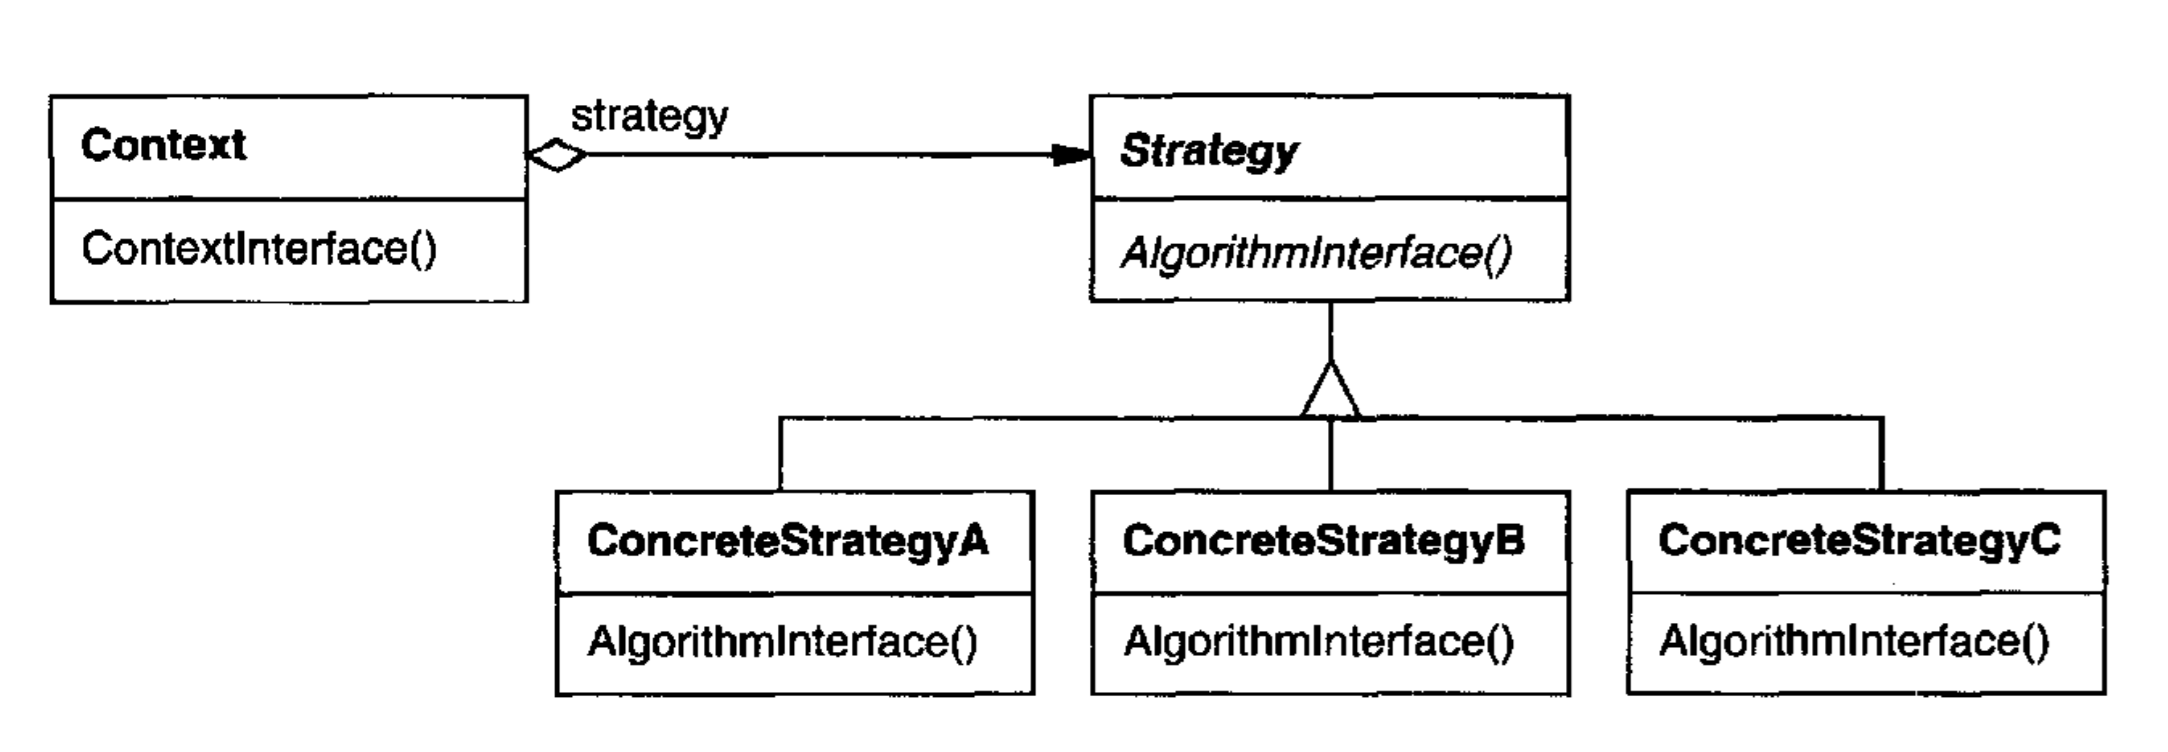
\includegraphics[width=\linewidth]{./figures/program/strategy.png}
  \caption{UML diagram for the Strategy design pattern from~\cite{DesignPatterns}}
\end{figure}

This is a great design pattern for research purposes since it facilitates experimentation with various algorithms for the same purpose. It also makes the code easily readable, as the Strategy interface provides an abstraction layer between the Context and the concrete implementation.

\section{Language choice}

With the specified goals and the architecture in mind, I needed a language that is object-oriented, easily readable by beginners and has extensive capabilities for using complex numbers, linear algebra and plotting. For these purposes, I choose the Python language. Python is concise, it reads like pseudocode and has libraries such as NumPy, SciPy and Matplotlib, and so on, covering all areas of data science. Furthermore, it is well-known and extensively used by researchers with no software engineering background, allowing for easier collaboration.

\section{High level design}

The source code of the software can be divided into three parts:

\begin{itemize}
    \item Graph models
    \item Simulators
    \item Running, configuration and result collection
\end{itemize}





\section{Gráfmodellek}

A félév során sokféle gráfon futtattam szimulációs kísérleteket, melyek során több problémába ütköztem. Kezdetben úgy oldottam meg a szimulációkat, hogy a célgráfok szomszédossági mátrixait generáltam le, egyben a memóriában tartva azokat és a lépések során a megfelelő csúcshoz tartozó sorokat lekérdezve.

Ezzel a módszerrel több probléma is jelentkezett. Az első gondot az okozta, hogy a szomszédossági mátrix mérete a csúcsszám négyzetével arányos, ezért pár ezer csúcsú gráfot már nem tudtam a memóriában tartva szimulálni. A második probléma pedig az volt, hogy a szomszédossági mátrixos ábrázolás nagyon távol esett az emberi szempontból természetes ábrázolástól. A kvantumbolyongásos szimulációkat tipikusan nem véletlenszerű gráfokon szokták kipróbálni, hanem jól ismert struktúrával rendelkező gráfokon. Ilyen gráfok például a ,,súlyzók''
vagy a ragasztott bináris fák.

A súlyzó gráf két egyforma méretű kört tartalmaz, mindkét körből kiválasztva $k - k$ darab csúcsot, melyek teljes páros gráfot alkotnak (a súlyzó középső rúdját). A körökben pedig nem csak az egymás melletti csúcsok között fut él, hanem futhat él minden $i.$ csúcs között is. A ragasztott bináris fában két egyforma méretű teljes bináris fa leveleit szembefordítjuk és a két oldali levelek közé egy teljes páros gráfot készítünk.

A fenti leírásból látható, hogy az ember számára természetes leírás a gráfokat ismert részgráfok kompozitjaként adja meg. A félév során olyan architektúrát alakítottam ki a szimulációkhoz, mely ezt a szemléletet támogatja. A szomszédossági mátrixos tárolási mód helyett pedig a szomszédossági orákulum megközelítést használva nagyban csökkent az alkalmazás memóriaigénye. Ennek a megközelítésnek a lényege, hogy az ismert struktúrájú gráfokra nem tárolok a memóriában szomszédossági információt, helyette biztosítok egy függvényt, amely a bemeneti paraméterként kapott csúcsindexre kiszámolja a vele szomszédos csúcsok indexeit.

A félév során a következő nevesített részgráfok szomszédossági orákulumját implementáltam:

\begin{itemize}
  \item BinaryTree
  \item Bipartite
  \item Circle
  \item Path
  \item Random
\end{itemize}

\change{Új: Hiperkocka}

\begin{center}
  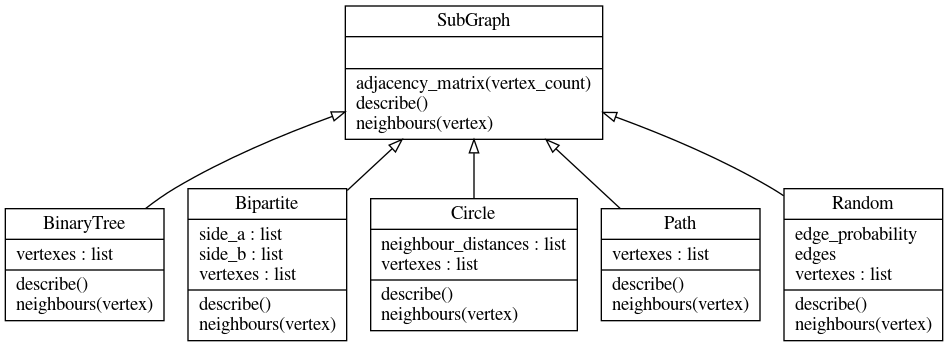
\includegraphics[width=\linewidth]{./figures/program/subgraph.png}
\end{center}

Ezen részgráfokból épülnek fel az alábbi kompozit gráfok:
\begin{itemize}
  \item Dumbbell
  \item GluedBinary
\end{itemize}

\begin{center}
  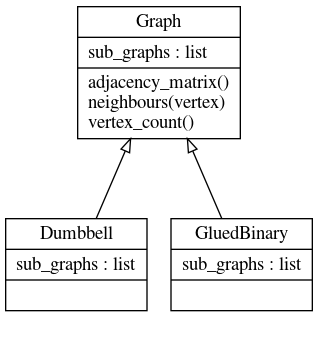
\includegraphics[width=0.4\linewidth]{./figures/program/graph.png}
\end{center}

\section{Szimulátorok}

A szimulátor osztályok közül a klasszikus tetszőleges kompozit gráfot tud
fogadni.

\change{Itt fontos átírni, hogy a kvantumszimulátor mostmár d-regulárist is tud!}

A kvantumszimulátor jelenleg a kvantumbolyongás egy speciális esetét, az egyenesen való bolyongást képes kezelni, mely a 2-regularitása miatt egyszerűbben implementálható. Hosszú távú cél a k-reguláris, illetve az általános gráfokra kiterjeszteni ezt a szimulátort.

\begin{center}
  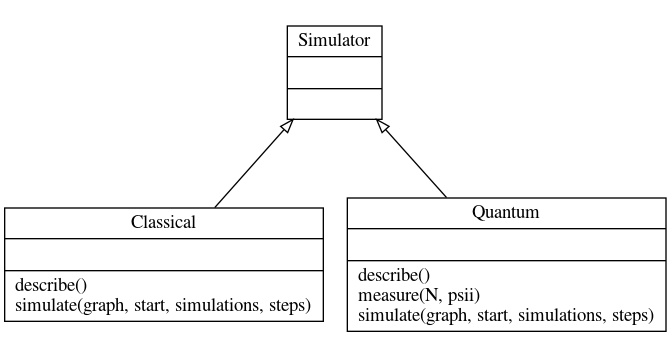
\includegraphics[width=0.8\linewidth]{./figures/program/simulator.png}
\end{center}

\section{Futtatás, konfiguráció, eredmények ábragenerátora}

\change{Itt van pár újdonság, pl. sajátértékek kiírása, stb.}

A fenti osztályok segítségével egy olyan keretrendszert alakítottam ki, melyben
nagyon gyorsan fel lehet 1-1 futtatást konfigurálni. A futtatás eredményeit egy
összesített Latex dokumentumba gyűjti a program. Ez tartalmazza a beadott gráf
részgráfjainak nevesített típusát, szomszédossági mátrixait, illetve a teljes
gráf szomszédossági mátrixát, valamint a szimulációk eloszlási eredményeit. A
következő fejezetben több ilyen ábrát is bemutatok.



Az első fázisban a szomszédossági mátrixot generáltam le teljesen. Ez nagyon sok memóriát használt, az unitér mátrix meg mégtöbbet, nagyon rosszul skálázódott. Lecseréltem spare mátrixokra, az már egy fokkal jobb.

\change{Mérés összehasonlítás: Mátrix, Spare mátrix, Orákulum grafikon.}

Ezután kipróbáltam a spare mátrixokat, de azok is picit sokak voltak, ugyan a gráfban sok a 0, de azért
így is nagyon skálázódott.

A legjobb megoldás az úgynevezett gráf orákulum volt. A gráf orákulum lényege, hogy nem tároljuk a szomszédossági mátrixot, helyette biztosítunk egy függvényt, mely on-the-fly a gráf adott csúcsindexét odaadva neki visszaadja hogy annak mik a szomszédai. A coin kis méretű, azt lehet tárolni (max fokszám * max fokszám), ezért azzal nem bajlódtam, bár éppen lehetne.
\chapter{Results}

\section{Walk on line}

\change{TODO hosszabb klasszikus séta kép meg valami leírás mindenhova}

\begin{figure}[H]
\centering
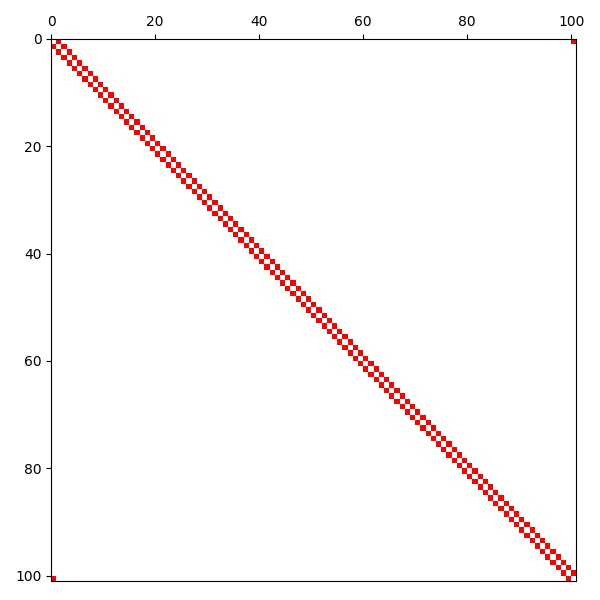
\includegraphics[width=0.5\linewidth]{./figures/results/path/graph.jpg}
\caption{Adjacency graph of the line}
\end{figure}

\begin{figure}[H]
  \centering
  \begin{subfigure}{.45\linewidth}
    \centering
    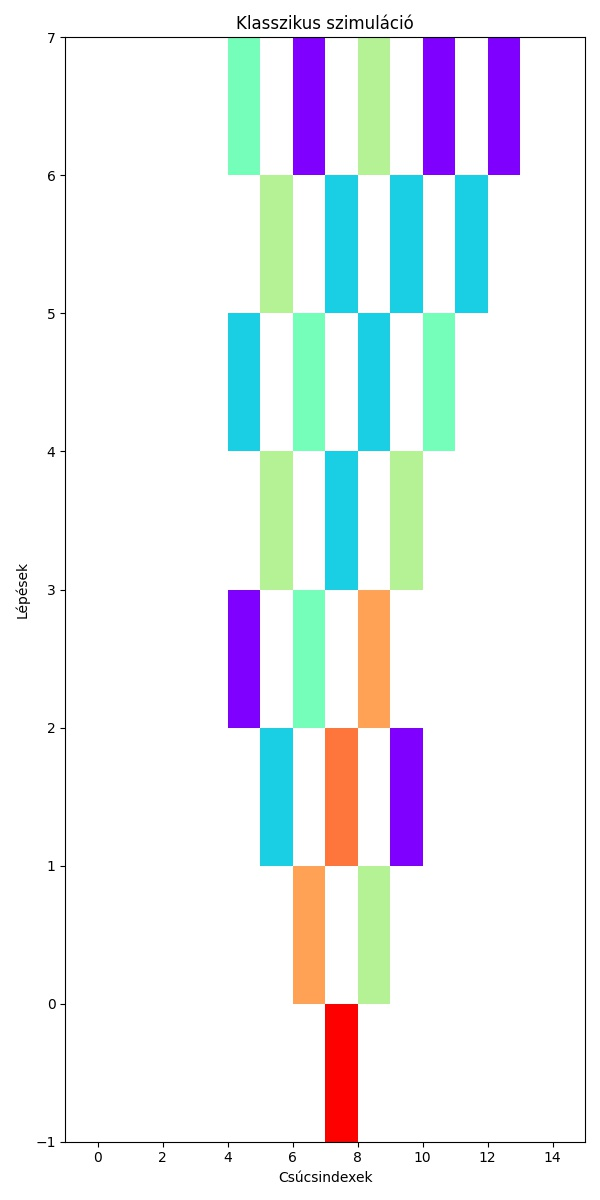
\includegraphics[width=\linewidth]{./figures/results/path/classical.jpg}
    \caption{Classical walk on the line}
  \end{subfigure}
  \begin{subfigure}{.45\linewidth}
    \centering
    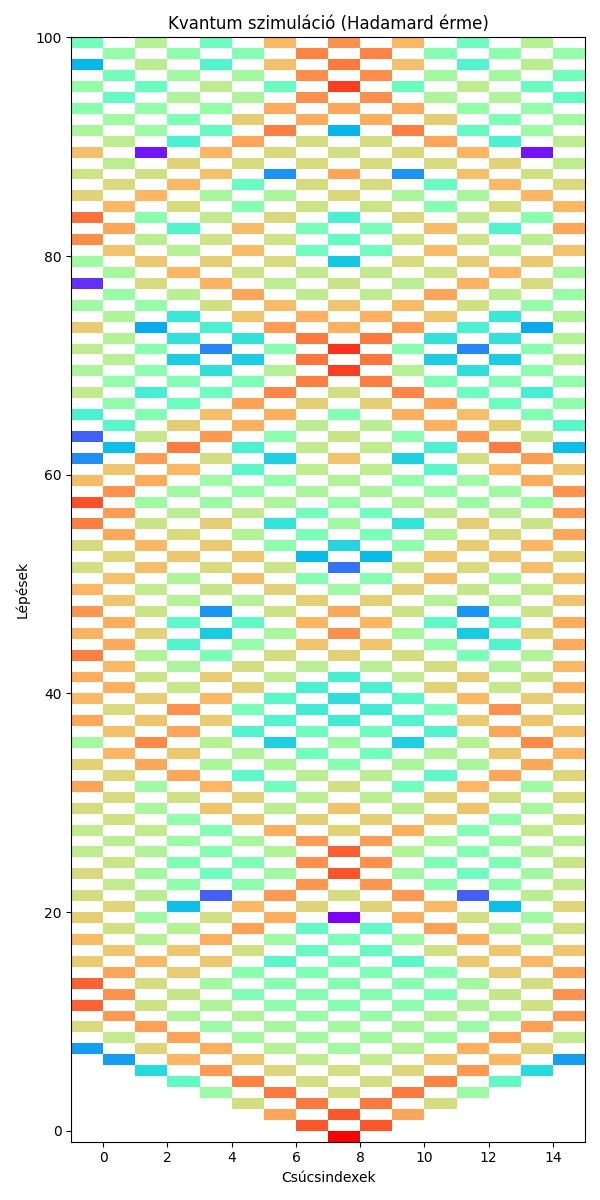
\includegraphics[width=\linewidth]{./figures/results/path/hadamard.jpg}
    \caption{Quantum walk on the line with the Hadamard coin}
  \end{subfigure}
  \caption{Walks on the line}
  \label{fig:all}
\end{figure}

\section{Walk on Grid}

\change{TODO: visszatérésről írni}

\begin{figure}[H]
\centering
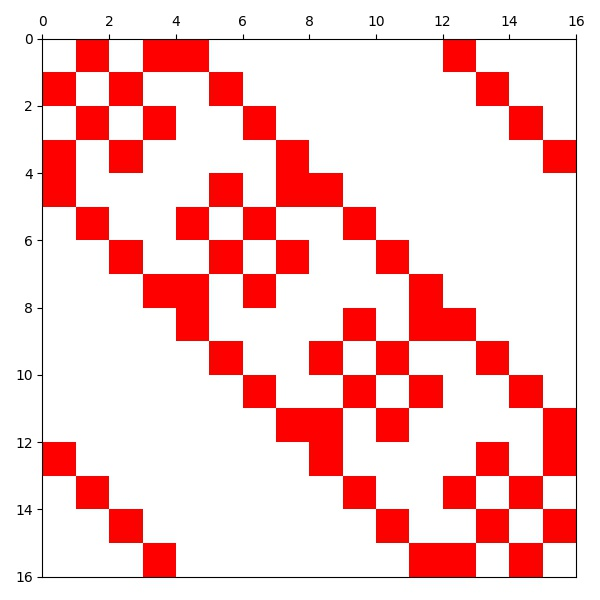
\includegraphics[width=0.5\linewidth]{./figures/results/grid/graph.jpg}
\caption{Adjacency graph of the grid}
\end{figure}

\begin{figure}[H]
  \centering
  \begin{subfigure}{.45\linewidth}
    \centering
    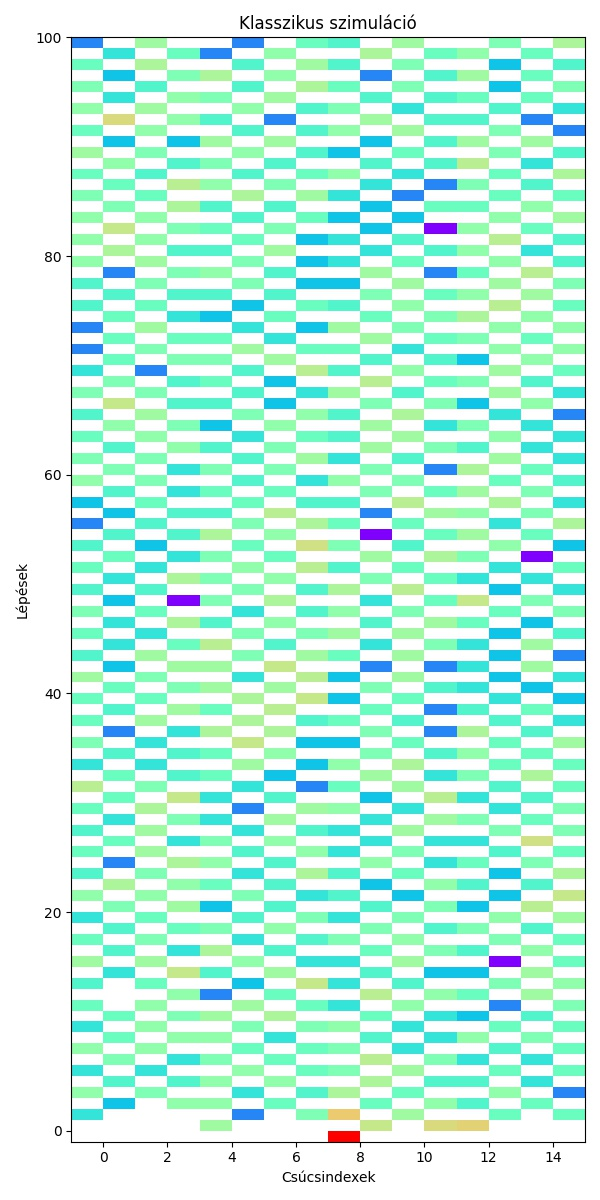
\includegraphics[width=\linewidth]{./figures/results/grid/classical.jpg}
    \caption{Classical walk on the grid}
  \end{subfigure}
  \begin{subfigure}{.45\linewidth}
    \centering
    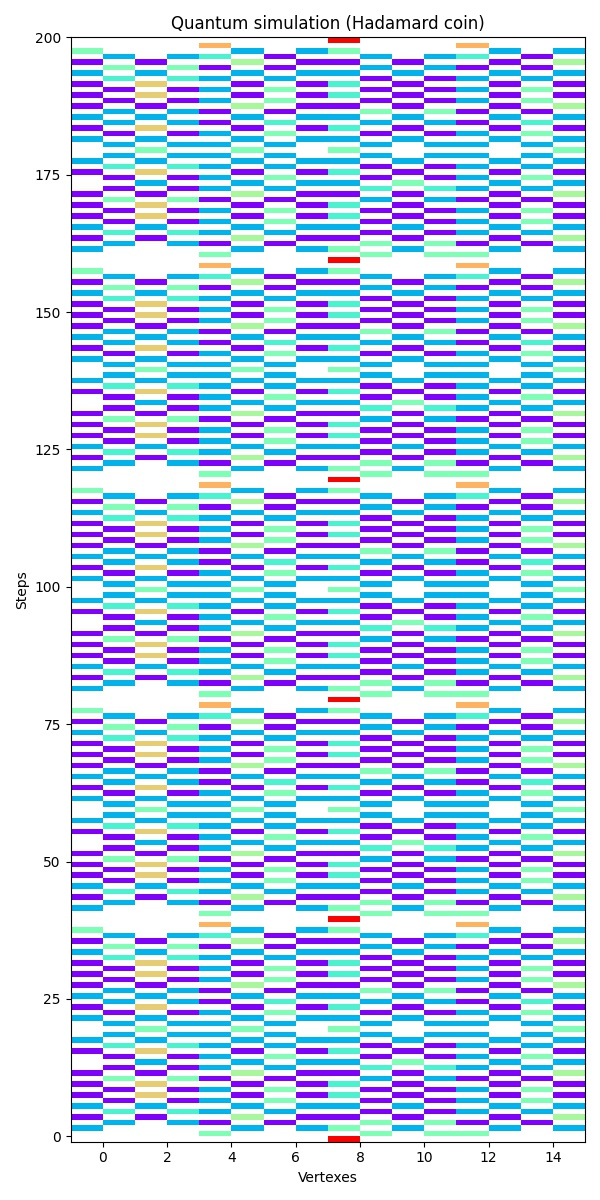
\includegraphics[width=\linewidth]{./figures/results/grid/hadamard.jpg}
    \caption{Quantum walk on the grid with the Hadamard coin}
  \end{subfigure}
  \caption{Walks on the grid}
  \label{fig:all}
\end{figure}

\begin{figure}[H]
  \centering
  \begin{subfigure}{.45\linewidth}
    \centering
    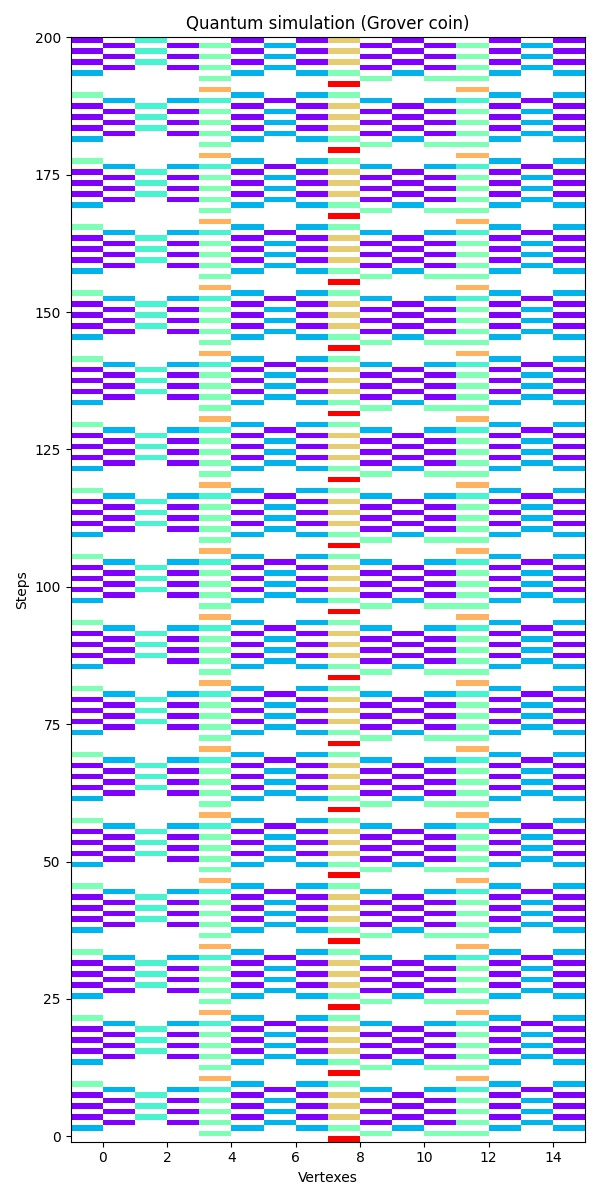
\includegraphics[width=\linewidth]{./figures/results/grid/grover.jpg}
    \caption{Quantum walk on the line with the Grover coin}
  \end{subfigure}
  \begin{subfigure}{.45\linewidth}
    \centering
    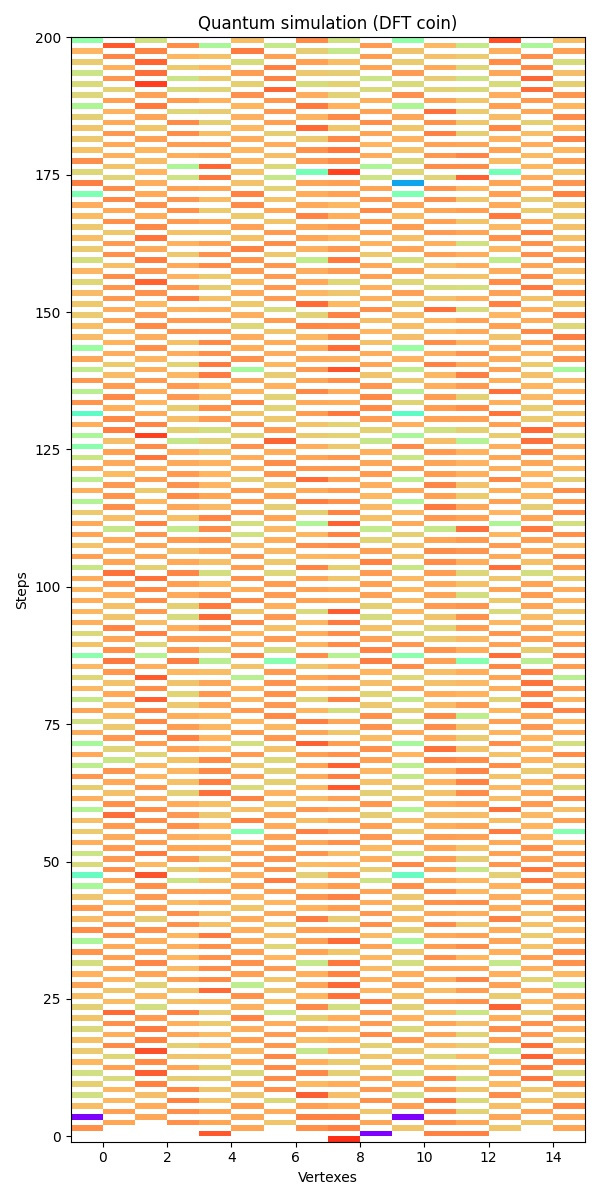
\includegraphics[width=\linewidth]{./figures/results/grid/dft.jpg}
    \caption{Quantum walk on the grid with the Fourier coin}
  \end{subfigure}
  \caption{Walks on the grid}
  \label{fig:all}
\end{figure}


\section{Walk on Hypercube}

\change{TODO: visszatérésről írni}

\begin{figure}[H]
\centering
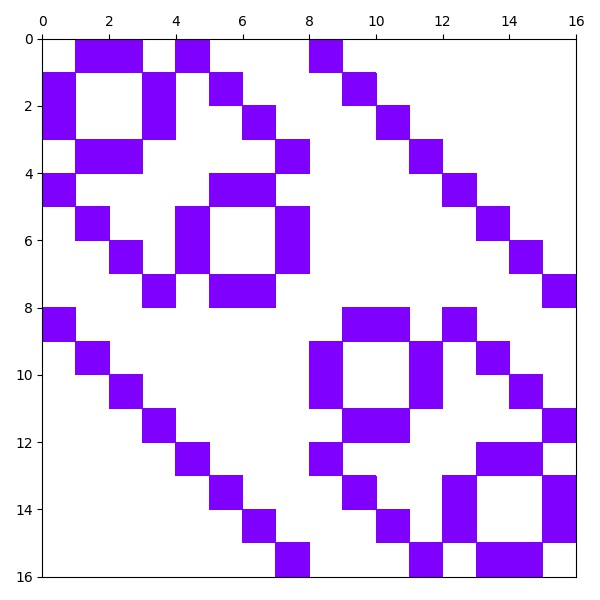
\includegraphics[width=0.5\linewidth]{./figures/results/hypercube/graph.jpg}
\caption{Adjacency graph of the hypercube}
\end{figure}

\begin{figure}[H]
  \centering
  \begin{subfigure}{.45\linewidth}
    \centering
    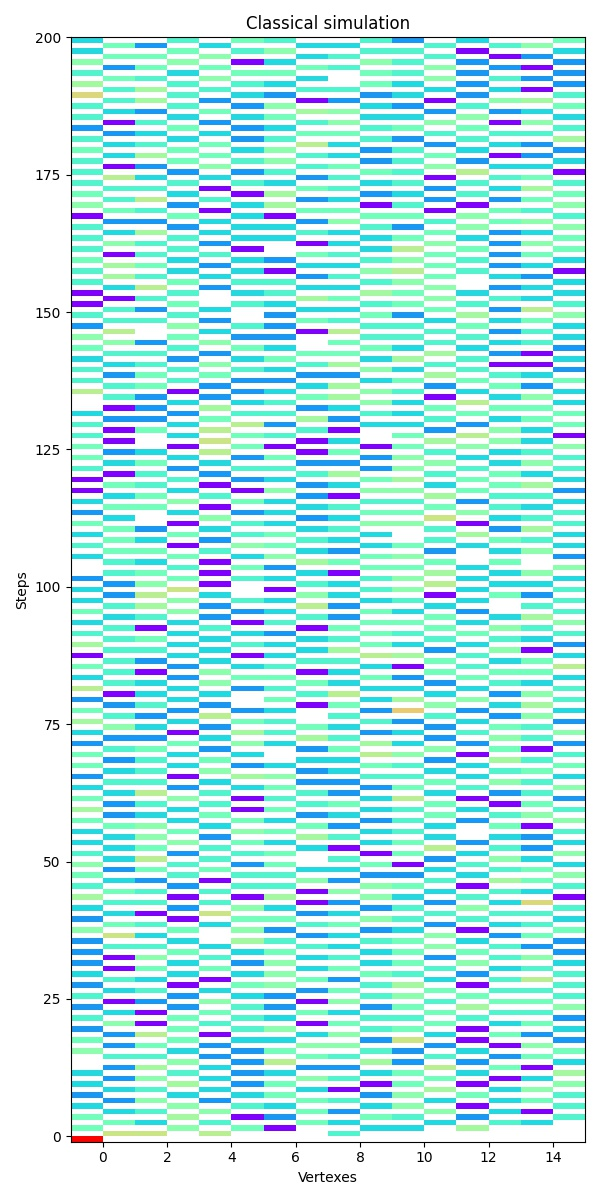
\includegraphics[width=\linewidth]{./figures/results/hypercube/classical.jpg}
    \caption{Classical walk on the hypercube}
  \end{subfigure}
  \begin{subfigure}{.45\linewidth}
    \centering
    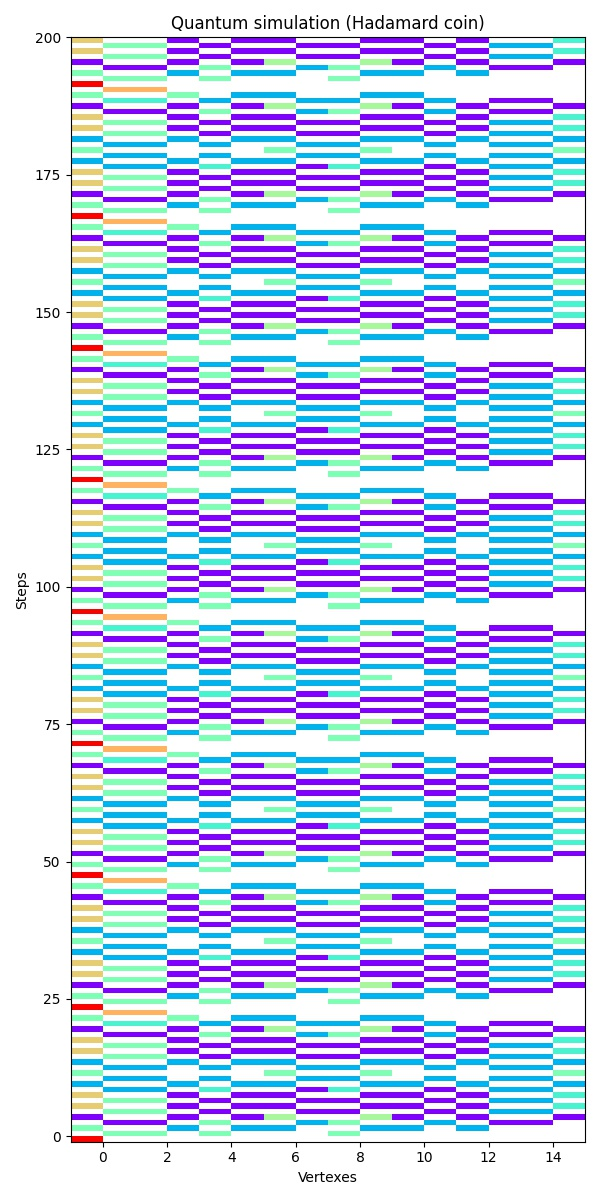
\includegraphics[width=\linewidth]{./figures/results/hypercube/hadamard.jpg}
    \caption{Quantum walk on the hypercube with the Hadamard coin}
  \end{subfigure}
  \caption{Walks on the hypercube}
  \label{fig:all}
\end{figure}

\begin{figure}[H]
  \centering
  \begin{subfigure}{.45\linewidth}
    \centering
    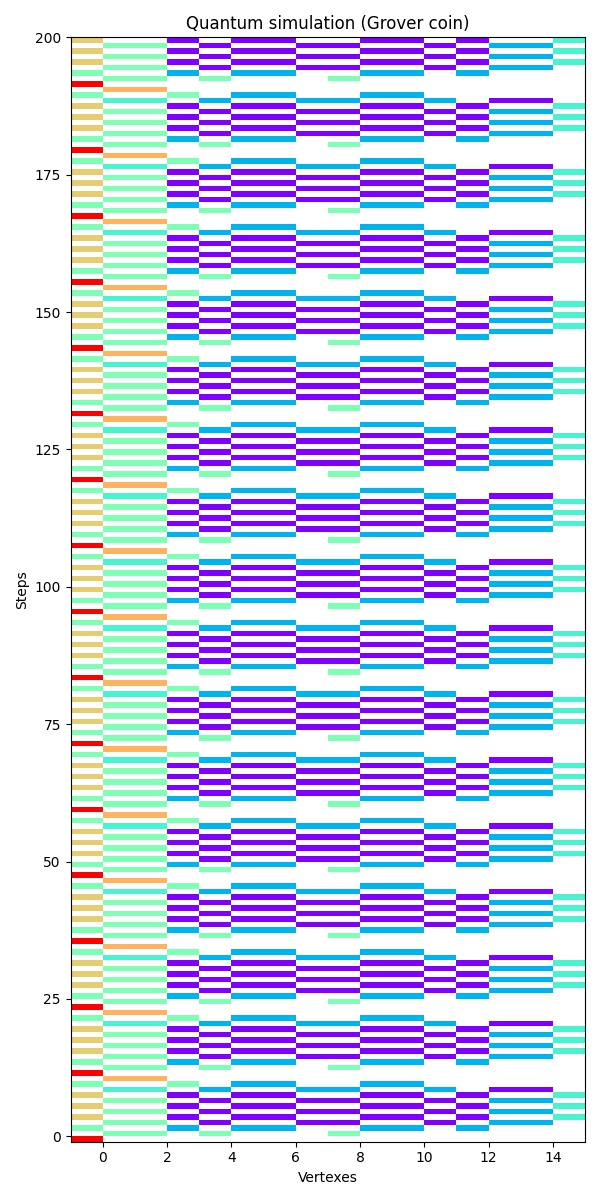
\includegraphics[width=\linewidth]{./figures/results/hypercube/grover.jpg}
    \caption{Quantum walk on the line with the Grover coin}
  \end{subfigure}
  \begin{subfigure}{.45\linewidth}
    \centering
    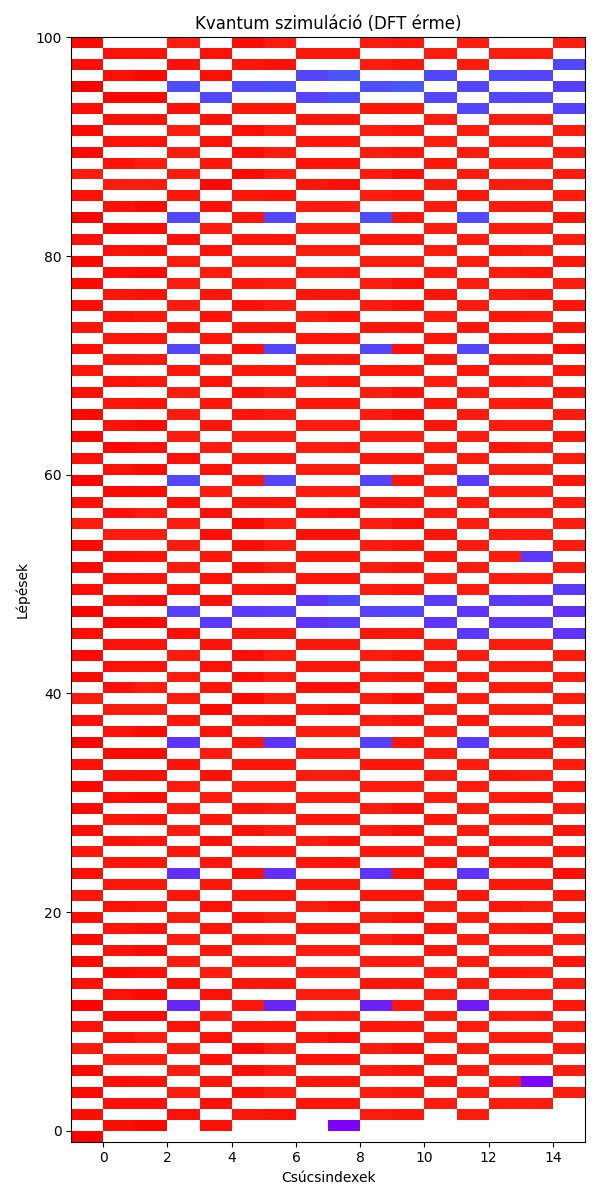
\includegraphics[width=\linewidth]{./figures/results/hypercube/dft.jpg}
    \caption{Quantum walk on the hypercube with the Fourier coin}
  \end{subfigure}
  \caption{Walks on the hypercube}
  \label{fig:all}
\end{figure}

\chapter*{\koszonetnyilvanitas}\addcontentsline{toc}{chapter}{\koszonetnyilvanitas}

Firstly, I would like to thank my advisor, dr.~Katalin Friedl, for her commitment to spending a significant amount of time with me, discussing my research both during the school year and over the summer. Without her supervision and mathematical expertise, this effort would not have been achievable.

Secondly, I would like to thank the Quantum Information National Laboratory for their continued support of quantum informatics research in our university.

% List of Figures, Tables
%\listoffigures\addcontentsline{toc}{chapter}{\listfigurename}
%\listoftables\addcontentsline{toc}{chapter}{\listtablename}

% Bibliography
\nocite{*}
\addcontentsline{toc}{chapter}{\bibname}
\bibliography{bib/mybib}

% Appendices
%----------------------------------------------------------------------------
\appendix
%----------------------------------------------------------------------------
\chapter*{\fuggelek}\addcontentsline{toc}{chapter}{\fuggelek}
\setcounter{chapter}{\appendixnumber}
%\setcounter{equation}{0} % a fofejezet-szamlalo az angol ABC 6. betuje (F) lesz
\numberwithin{equation}{section}
\numberwithin{figure}{section}
\numberwithin{lstlisting}{section}
%\numberwithin{tabular}{section}


\section{Első függelék}
\begin{figure}[!ht]
\centering
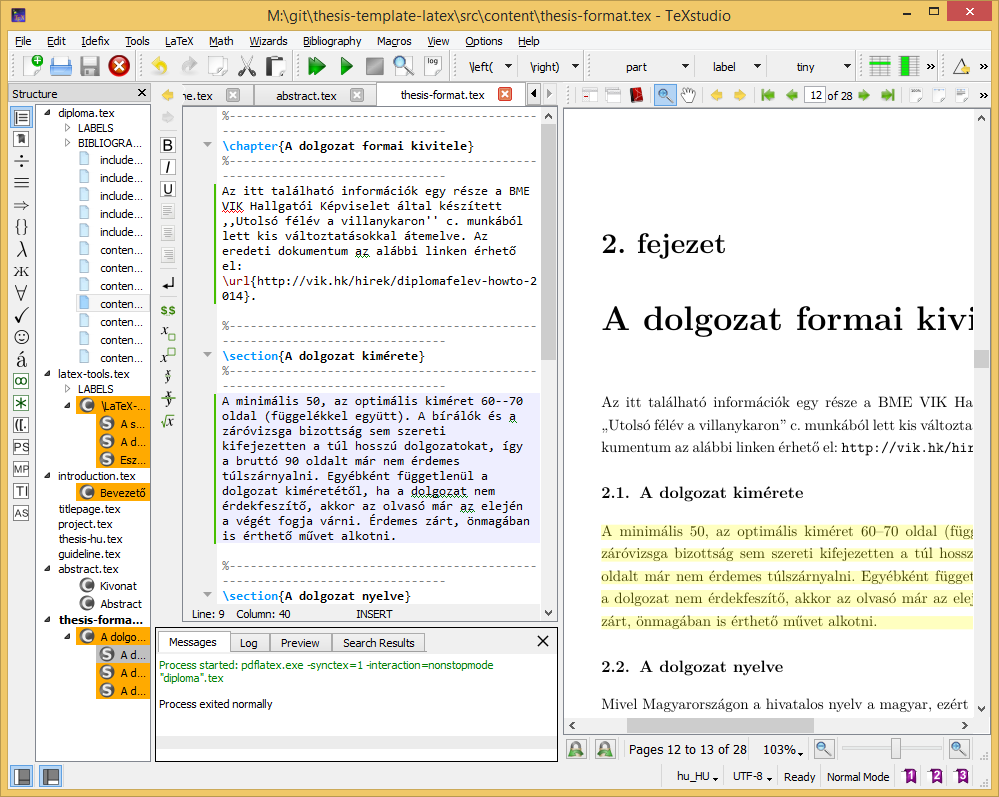
\includegraphics[width=150mm, keepaspectratio]{figures/TeXstudio.png}
\caption{A TeXstudio \LaTeX-szerkesztő.} 
\end{figure}

\clearpage

%----------------------------------------------------------------------------
\section{Második függelék}
%----------------------------------------------------------------------------
A Pitagorasz-tételből levezetve
\begin{align}
c^2=a^2+b^2=42.
\end{align}
A Faraday-indukciós törvényből levezetve
\begin{align}
\rot E=-\frac{dB}{dt}\hspace{1cm}\longrightarrow \hspace{1cm}
U_i=\oint\limits_\mathbf{L}{\mathbf{E}\mathbf{dl}}=-\frac{d}{dt}\int\limits_A{\mathbf{B}\mathbf{da}}=42.
\end{align}


\end{document}
